%Version 3 October 2023
% See section 11 of the User Manual for version history
%
%%%%%%%%%%%%%%%%%%%%%%%%%%%%%%%%%%%%%%%%%%%%%%%%%%%%%%%%%%%%%%%%%%%%%%
%%                                                                 %%
%% Please do not use \input{...} to include other tex files.       %%
%% Submit your LaTeX manuscript as one .tex document.              %%
%%                                                                 %%
%% All additional figures and files should be attached             %%
%% separately and not embedded in the \TeX\ document itself.       %%
%%                                                                 %%
%%%%%%%%%%%%%%%%%%%%%%%%%%%%%%%%%%%%%%%%%%%%%%%%%%%%%%%%%%%%%%%%%%%%%

%%\documentclass[referee,sn-basic]{sn-jnl}% referee option is meant for double line spacing

%%=======================================================%%
%% to print line numbers in the margin use lineno option %%
%%=======================================================%%

%%\documentclass[lineno,sn-basic]{sn-jnl}% Basic Springer Nature Reference Style/Chemistry Reference Style

%%======================================================%%
%% to compile with pdflatex/xelatex use pdflatex option %%
%%======================================================%%

%%\documentclass[pdflatex,sn-basic]{sn-jnl}% Basic Springer Nature Reference Style/Chemistry Reference Style


%%Note: the following reference styles support Namedate and Numbered referencing. By default the style follows the most common style. To switch between the options you can add or remove “Numbered” in the optional parenthesis. 
%%The option is available for: sn-basic.bst, sn-vancouver.bst, sn-chicago.bst%  
 
%%\documentclass[sn-nature]{sn-jnl}% Style for submissions to Nature Portfolio journals
%%\documentclass[sn-basic]{sn-jnl}% Basic Springer Nature Reference Style/Chemistry Reference Style
\documentclass[sn-mathphys-num]{sn-jnl}% Math and Physical Sciences Numbered Reference Style 
%%\documentclass[sn-mathphys-ay]{sn-jnl}% Math and Physical Sciences Author Year Reference Style
%%\documentclass[sn-aps]{sn-jnl}% American Physical Society (APS) Reference Style
%%\documentclass[sn-vancouver,Numbered]{sn-jnl}% Vancouver Reference Style
%%\documentclass[sn-apa]{sn-jnl}% APA Reference Style 
%%\documentclass[sn-chicago]{sn-jnl}% Chicago-based Humanities Reference Style

%%%% Standard Packages
%%<additional latex packages if required can be included here>

\usepackage{graphicx}%
\usepackage{multirow}%
\usepackage{amsmath,amssymb,amsfonts}%
\usepackage{amsthm}%
\usepackage{mathrsfs}%
\usepackage[title]{appendix}%
\usepackage{xcolor}%
\usepackage{textcomp}%
\usepackage{manyfoot}%
\usepackage{booktabs}%
\usepackage{algorithm}%
\usepackage{algorithmicx}%
\usepackage{algpseudocode}%
\usepackage{listings}%
%%%%

%%%%%=============================================================================%%%%
%%%%  Remarks: This template is provided to aid authors with the preparation
%%%%  of original research articles intended for submission to journals published 
%%%%  by Springer Nature. The guidance has been prepared in partnership with 
%%%%  production teams to conform to Springer Nature technical requirements. 
%%%%  Editorial and presentation requirements differ among journal portfolios and 
%%%%  research disciplines. You may find sections in this template are irrelevant 
%%%%  to your work and are empowered to omit any such section if allowed by the 
%%%%  journal you intend to submit to. The submission guidelines and policies 
%%%%  of the journal take precedence. A detailed User Manual is available in the 
%%%%  template package for technical guidance.
%%%%%=============================================================================%%%%

%% as per the requirement new theorem styles can be included as shown below
\theoremstyle{thmstyleone}%
\newtheorem{theorem}{Theorem}%  meant for continuous numbers
%%\newtheorem{theorem}{Theorem}[section]% meant for sectionwise numbers
%% optional argument [theorem] produces theorem numbering sequence instead of independent numbers for Proposition
\newtheorem{proposition}[theorem]{Proposition}% 
%%\newtheorem{proposition}{Proposition}% to get separate numbers for theorem and proposition etc.

\theoremstyle{thmstyletwo}%
\newtheorem{example}{Example}%
\newtheorem{remark}{Remark}%

\theoremstyle{thmstylethree}%
\newtheorem{definition}{Definition}%

\raggedbottom
%%\unnumbered% uncomment this for unnumbered level heads

\begin{document}

\title[The Opportunity Gap and Equity in Education]{The Opportunity Gap and Equity in Education: The Effects of Advanced Placement Course Participation on College Readiness and Success}

%%=============================================================%%
%% GivenName	-> \fnm{Joergen W.}
%% Particle	-> \spfx{van der} -> surname prefix
%% FamilyName	-> \sur{Ploeg}
%% Suffix	-> \sfx{IV}
%% \author*[1,2]{\fnm{Joergen W.} \spfx{van der} \sur{Ploeg} 
%%  \sfx{IV}}\email{iauthor@gmail.com}
%%=============================================================%%

\author[1,2]{\fnm{Khanh} \sur{Ho}}\email{khanhho5813@gmail.com}

\author[2]{\fnm{Priya} \sur{Prasad}}\email{Priya.Prasad@utsa.edu}
%\equalcont{These authors contributed equally to this work.}

\author[2]{\fnm{Tina} \sur{Vega}}\email{Tina.Vega@utsa.edu}
%\equalcont{These authors contributed equally to this work.}

\author[2]{\fnm{David} \sur{Risk-Mora}}\email{david.risk@utsa.edu}

\author[2]{\fnm{Paula} \sur{Jaimes-Buitron}}\email{paula.jaimesbuitron@utsa.edu}

\author*[2]{\fnm{Juan B.} \sur{Gutiérrez}}\email{juan.gutierrez3@utsa.edu}
%\equalcont{These authors contributed equally to this work.}

\affil[1]{\orgdiv{Department}, \orgname{Organization}, \orgaddress{\street{Street}, \city{San Antonio}, \postcode{78249}, \state{Texas}, \country{USA}}}

\affil*[2]{\orgdiv{Department of Mathematics}, \orgname{University of Texas at San Antonio}, \orgaddress{\street{1 UTSA Cir}, \city{San Antonio}, \postcode{78249}, \state{Texas}, \country{USA}}}

\affil[3]{\orgdiv{Department}, \orgname{Organization}, \orgaddress{\street{Street}, \city{City}, \postcode{610101}, \state{State}, \country{Country}}}

%%==================================%%
%% Sample for unstructured abstract %%
%%==================================%%

\abstract{    Although the benefits of enrolling in Advanced Placement (AP) courses are clear and ideally, every student should have access to and excel in these courses, the reality paints a different picture. Arbitrary factors such as race, ethnicity, ZIP code, and socioeconomic status, collectively known as the opportunity gap, often dictate individuals' educational paths and perpetuate disparities in access to rigorous academic offerings. By utilizing publicly available datasets from the Civil Rights Data Collection (CRDC) and the U.S. Bureau of the Census' Small Area Income and Poverty Estimates (SAIPE) program, alongside specific data from the University of Texas at San Antonio, this research aims to provide a detailed and nuanced understanding of how economic and demographic factors influence educational opportunities. The analysis reveals a significant positive correlation between AP course participation and higher college GPAs, suggesting that students who engage in AP coursework are better prepared for academic challenges in higher education. However, the study finds no statistically significant association between AP participation and college graduation rates. %, indicating that additional factors influence long-term academic success. 
Furthermore, the comparative analysis of the relationship between the proportion of children aged 5-17 living in poverty and enrollment in AP courses in Texas reveals substantial disparities linked to socioeconomic status. Higher poverty rates are associated with lower AP enrollment rates, particularly in math and science. Overall, the findings underscore the critical importance of addressing the opportunity gap to promote educational equity and excellence. By implementing targeted interventions and fostering a supportive and inclusive educational environment, we can ensure that all students, regardless of their socioeconomic background, have the opportunity to achieve their full potential and succeed in their academic and professional pursuits.}

%%================================%%
%% Sample for structured abstract %%
%%================================%%

% \abstract{\textbf{Purpose:} The abstract serves both as a general introduction to the topic and as a brief, non-technical summary of the main results and their implications. The abstract must not include subheadings (unless expressly permitted in the journal's Instructions to Authors), equations or citations. As a guide the abstract should not exceed 200 words. Most journals do not set a hard limit however authors are advised to check the author instructions for the journal they are submitting to.
% 
% \textbf{Methods:} The abstract serves both as a general introduction to the topic and as a brief, non-technical summary of the main results and their implications. The abstract must not include subheadings (unless expressly permitted in the journal's Instructions to Authors), equations or citations. As a guide the abstract should not exceed 200 words. Most journals do not set a hard limit however authors are advised to check the author instructions for the journal they are submitting to.
% 
% \textbf{Results:} The abstract serves both as a general introduction to the topic and as a brief, non-technical summary of the main results and their implications. The abstract must not include subheadings (unless expressly permitted in the journal's Instructions to Authors), equations or citations. As a guide the abstract should not exceed 200 words. Most journals do not set a hard limit however authors are advised to check the author instructions for the journal they are submitting to.
% 
% \textbf{Conclusion:} The abstract serves both as a general introduction to the topic and as a brief, non-technical summary of the main results and their implications. The abstract must not include subheadings (unless expressly permitted in the journal's Instructions to Authors), equations or citations. As a guide the abstract should not exceed 200 words. Most journals do not set a hard limit however authors are advised to check the author instructions for the journal they are submitting to.}

\keywords{keyword1, Keyword2, Keyword3, Keyword4}

%%\pacs[JEL Classification]{D8, H51}

%%\pacs[MSC Classification]{35A01, 65L10, 65L12, 65L20, 65L70}

\maketitle

%%%%%%%%%%%%%%%%%%%%%%%%%%%%%%%%%%%%%%%%%%%%%%%%%%%%%%%%%%%%%%
\section{Introduction}\label{sec:Intro}

The purpose of this manuscript is to investigate the presence of an opportunity gap among students in accessing advanced placement courses and its potential impact on their performance and persistence at the college level. We ask the following questions:\\
\begin{enumerate}
    \item How does socioeconomic status contribute to disparities in access to advanced placement courses among high school students?
    \item How does participation in advanced placement courses in high school correlate with students' academic performance in college?\\
\end{enumerate}

The Advanced Placement (AP) program originated in the 1950s with funding from the Fund for the Advancement of Education of the Ford Foundation \cite{curtis2002learning, diyanni2002origins}. Initially established through two projects, it was later assumed by the College Board in 1955, officially becoming the Advanced Placement Program \cite{curtis2002learning, diyanni2002origins}. Since then, the AP program has effectively provided students with the opportunity to engage in university-level coursework during their secondary/high school years \cite{curtis2002learning, diyanni2002origins}. Presently, with AP courses available in numerous subjects, approximately 35$\%$ of recent high school graduates have taken at least one AP course during their high school \cite{apreport23}. Giving students the access to the realm of AP courses can offer a myriad of advantages that extend far beyond the confines of the high school classroom \cite{apreport}.\\ 

Firstly, participation in AP courses aids students in the college admission process \cite{curtis2002learning, diyanni2002origins}. AP courses carry greater weight in GPA (Grade Point Average) calculations compared to standard courses, offering students who excel in AP classes a substantial GPA boost \cite{collegeoutcomescomparison}. Achieving a higher GPA translates to a better rank, which proves highly advantageous for students \cite{curtis2002learning}. Particularly in Texas, the Top 10 Percent Law (officially known as House Bill 588, section 51.803a) guarantees automatic admission to all state-funded universities for Texas students who graduated in the top ten percent of their high school class \cite{texas_legislation}. Engaging in advanced coursework can prove advantageous for college applications, particularly when students achieve qualifying scores (three or higher) on AP exams, as these higher grades can enhance their competitiveness for admission to selective colleges\cite{geiser2004role}. Furthermore, many colleges and universities recognize the rigor of AP coursework by offering college credit or advanced placement to students who perform well on AP exams \cite{diyanni2002origins}. By earning college credits through AP courses, students can potentially accelerate their progress towards degree completion, reducing the overall cost of tuition and shortening the time needed to graduate \cite{curtis2002learning, collegeoutcomescomparison}.\\

Secondly, participation in AP courses not only prepares students for the academic rigors of college but also facilitates a smoother transition to higher education, ultimately increasing their likelihood of college enrollment and successful degree attainment \cite{long2012effects, ackerman2013high, gurantz2021college, geiser2004role}. AP courses provide students with an opportunity to engage in rigorous academic content comparable to introductory college-level courses \cite{apreport, curtis2002learning}. The curriculum and organization of AP courses, along with the learning opportunities they present to high school students, can serve as fundamental elements contributing to success in higher education \cite{curtis2002learning}. Research by Long et al. \cite{long2012effects} showed that students who take rigorous courses before graduating from high school are more likely to enroll in college, particularly in four-year institutions, compared to those who do not. Similarly, Ackerman et al.  \cite{ackerman2013high} analyzed data from 1999 to 2009 at the Georgia Institute of Technology (Georgia Tech) and found a correlation between participation in AP exams and higher college graduation rates. Participation in AP courses and an increasing number of AP exams with qualifying grades (3 or higher) were found to correlate with higher college graduation rates compared to students who did not complete any AP exams \cite{ackerman2013high}. Additionally, students achieving higher scores on AP exams tend to demonstrate better performance in college\cite{geiser2004role, ackerman2013high}.\\

Although the benefits of enrolling in AP courses are clear, and ideally, every student should have access to and excel in these courses, the reality paints a different picture. The disparities in access to AP courses persist not only within schools but also among different school districts, highlighting the significant impact on students' ability to enroll in advanced coursework  \cite{solorzano2002critical, colgren2015closing}. Within schools, data has revealed significant discrepancies in AP course enrollment rates among students of different racial backgrounds, often resulting in what has been described as 'Schools within Schools' \cite{solorzano2002critical}. This phenomenon underscores the entrenched inequities within the education system, where certain groups of students are disproportionately excluded from accessing advanced coursework, thereby perpetuating systemic disparities in academic achievement and opportunities \cite{solorzano2002critical}. The same problem also happen among school districts, where variations in AP course availability and enrollment rates based on factors such as district wealth and demographics \cite{carter2013closing}. These disparities reflect systemic inequities within the education system, perpetuating barriers to academic opportunities for certain groups of students \cite{carter2013closing}.\\

The arbitrary factors such as race, ethnicity, ZIP code, and socioeconomic status are know as the opportunity gap, which often dictate individuals' educational paths and perpetuate disparities in access to rigorous academic offerings \cite{carter2013closing}. The term ``opportunity gap" sheds light on the challenges and barriers that young students encounter during their educational journeys \cite{carter2013closing}. Carter and Welner vividly portrays the profound impact of the opportunity gap on students, stating: 
\begin{quote}Vast opportunity gaps limit children's future prospects every day in schools in almost every community across America. Talent is being wasted, particularly among those living in poverty and in disadvantaged communities of color. Children in these communities are not reaching their full potential and are not ``closing the gap" in achievement - precisely because they are not receiving equitable and meaningful opportunities to reach that potential. \cite{carter2013closing}
\end{quote}

The influence of income level and socioeconomic status on students' success remains substantial, reflecting the pervasive impact of the opportunity gap on educational outcomes \cite{whither_opportunity, klugman2012resource, ladson2006achievement, carter2013closing}. Being born into families of higher socioeconomic status often ensures better access to quality education \cite{carter2013closing, whither_opportunity, orfield2006vicious}. As family income rises, so do expenditures on enrichment activities such as music and art lessons, tutoring, and educational materials \cite{whither_opportunity, carter2013closing}. Beyond financial resources, high-income families also benefit from a wealth of social and familial support \cite{whither_opportunity, klugman2012resource}. Drawing from data obtained in the Educational Longitudinal Study of 2002 (ELS), a comprehensive study encompassing a nationally representative sample of tenth graders in the United States, followed up in 2004 and 2006, it becomes evident that students attending private high schools or those located in affluent neighborhoods possess distinct advantages, including increased opportunities for admission to selective colleges \cite{klugman2012resource}. This advantage is deeply entrenched within the structural framework of the U.S. secondary school system, allowing affluent parents to strategically navigate educational opportunities for their children, such as enrollment in AP classes and achieving higher ACT/SAT scores—criteria highly valued in college admissions processes \cite{klugman2012resource, carter2013closing}. Consequently, these parents invest significant resources in selecting high schools that offer avenues to nurture such advantages, perpetuating a cycle of privilege and opportunity that exacerbates existing social and economic disparities within the educational landscape \cite{klugman2012resource, carter2013closing}.\\

Segregated housing is a consequence of both income disparities and racial inequality, exacerbating the issue of the opportunity gap \cite{carter2013closing, orfield2006vicious}. Orfield and McArdle  \cite{orfield2006vicious} elucidated that ``housing determines a family's location, making it the linchpin of opportunity, intertwined with numerous factors critical to the success of adults and children in American society." While many Americans believe that access to housing is equitable and reflects their hard work, the reality is that the prevailing patterns of housing segregation and the workings of the housing market are not solely dictated by economics or individual preferences \cite{orfield2006vicious, carter2013closing, pattillo2018black}.\\

Housing location plays a pivotal role in determining the quality of schools \cite{orfield2006vicious}. Residential sorting, driven by land use controls, results in some schools where the majority of students come from affluent backgrounds and have access to supplementary educational opportunities \cite{orfield2006vicious}. These schools often have reputation of high average test scores, largely influenced by students' advantageous starting positions, including family socioeconomic status, parental education levels, and peer group influences \cite{orfield2006vicious}. These high scores are then actively promoted by the real estate industry and communities as evidence of educational excellence, attracting more high-income families to the area \cite{orfield2006vicious}. Every parent desires for their children to reside in a favorable neighborhood and attend high-quality schools to set them up for success in life, and this aspiration extends to Black, Latino, and other minority families \cite{carter2013closing, pattillo2018black}. However, they frequently encounter discrimination in the housing market, even as middle-class families \cite{carter2013closing, orfield2006vicious, pattillo2018black}. Purchasing homes in so-called ``quality neighborhoods" can be arduous \cite{orfield2006vicious}. The lack of access to these neighborhoods means that these children are already at a disadvantage by attending schools with fewer resources and lower quality education \cite{orfield2006vicious, carter2013closing, pattillo2018black}. Consequently, the resultant segregation in education is not a matter of choice but an involuntary outcome of systemic inequalities\cite{carter2013closing, orfield2006vicious}.\\

School funding primarily comes from a combination of state, local, and federal sources \cite{texas_tribune_school_funding, hanushek2009schoolhouses}. Districts first rely on local property tax revenue to cover their base budgets, with the state providing the remaining balance \cite{hanushek2009schoolhouses}. Typically, state and local funding make up at least 90 percent of the total \cite{hanushek2009schoolhouses}. This reliance on state and local funding leads to significant disparities between districts \cite{carter2013closing, orfield2006vicious, hanushek2009schoolhouses}. School districts with substantial property wealth can generate more tax revenue for their schools compared to property-poor districts, even if they levy the same tax rate \cite{hanushek2009schoolhouses}. Despite efforts to secure additional funding from various sources, including state, federal, and philanthropic sources, urban school districts serving marginalized communities continue to struggle to compete with wealthier districts in terms of teacher salaries and resource allocation \cite{wilkins2006yes, wiener2007opportunity, carter2013closing}. These ongoing challenges in securing adequate funding and resources underscore the entrenched inequities within the education system, where socioeconomic factors significantly influence the distribution of resources and the quality of education provided to students \cite{carter2013closing, hanushek2009schoolhouses}.\\

In Texas, the story of school funding is intricate and multifaceted. Since 1993, the controversial ``Robin Hood" or recapture program has redistributed excess funding from wealthier districts to poorer ones \cite{texas_tribune_school_funding, texas_standard_school_funding}. To equalize funding across property-poor and property-wealthy districts, state sales tax, local property tax, and money collected through recapture are pooled together \cite{texas_standard_school_funding}. Then, a formula is used to determine how much money each student in public schools receives \cite{texas_standard_school_funding, texas_tribune_school_funding}. If districts collect more in property tax than the formula allows, the state takes the excess and uses it to fund other schools \cite{texas_standard_school_funding, texas_tribune_school_funding}. This means when property values increase, public schools do not get more money; they just receive less state funding \cite{texas_standard_school_funding, texas_tribune_school_funding}. While this system aims to level the playing field, it often leaves wealthier districts feeling overburdened and poorer districts still underfunded \cite{texas_standard_school_funding, texas_tribune_school_funding}. The frustration of wealthier school districts with the recapture program led to another unfair element called Golden Pennies \cite{texas_standard_school_funding}. Golden Pennies, created in 2006 after property-wealthy districts sued the state, are exempt from recapture \cite{texas_standard_school_funding}. They allow districts to increase their tax rate without being subject to recapture, letting them keep all the revenue collected \cite{texas_standard_school_funding}. This provides a significant advantage to districts with high property wealth but few students, with some collecting up to \$35,000 per student in Golden Pennies alone \cite{texas_standard_school_funding}. Complicating the situation further is the introduction of automatic tax compression in 2019 as part of the state’s education overhaul \cite{texas_standard_school_funding}. This policy reduces the property tax rate for every school district annually, setting new maximum rates based on the growth of property values within the district \cite{texas_standard_school_funding}. While intended to provide tax relief, this measure has eroded a key component of equity that the recapture system sought to address, as it allows districts with rapidly growing property values to benefit disproportionately \cite{texas_standard_school_funding}. Critics argue that automatic tax compression could undermine public school funding by shrinking the state's largest revenue source for education, potentially leading to calls for the elimination of school property taxes altogether \cite{texas_standard_school_funding}.\\

Schools serving predominantly low-income and minority students also grapple with issues of teacher quality even though students should have access to qualified educators to foster academic success \cite{wilkins2006yes, monitoring_school_quality, carter2013closing, orfield2006vicious}. According to Wilkins, classes in schools primarily serving children of color are twice as likely to be taught by inexperienced teachers compared to those serving predominantly White students \cite{wilkins2006yes}. Additionally, the analysis report by Mayer et al. \cite{monitoring_school_quality} also showed that the percentage of inexperienced teachers in low poverty schools was 11$\%$ whereas in high poverty schools it was 20 $\%$. The disparity in funding allocation poses a significant challenge in retaining high-quality educators \cite{wilkins2006yes, wiener2007opportunity}. Additionally, teachers also tend to gravitate towards schools with lower proportions of Black and low-achieving students \cite{whither_opportunity}. This stark reality underscores how students in need of greater educational support often receive less assistance than they require \cite{carter2013closing}.\\

Simply equalizing participation in rigorous courses, such as AP programs, does not suffice to address the persistent opportunity gaps observed between Black/White, Latino/White, and low-income/non-low-income students \cite{colgren2015closing, flores2007examining}. A study utilizing secondary data from the Illinois State Board of Education revealed that the curriculum and instruction of these courses tend to favor White and non-low-income students, resulting in unequal outcomes \cite{colgren2015closing}. The data demonstrated significant disparities in ACT scores between students who completed AP courses and those who did not, with the discrepancies notably larger among White students compared to Black and Latino students \cite{colgren2015closing}. While participation in AP courses benefits all students to some extent, the notably higher mean differences in scores for White students suggest that they derive greater advantages from these courses compared to their Black and Latino peers \cite{colgren2015closing}. This disparity highlights that simply increasing participation in rigorous courses without addressing underlying structural biases may only reinforce existing inequalities in academic achievement \cite{flores2007examining, colgren2015closing}.\\

Having outlined the significance of the opportunity gap and the disparities in access to AP courses, this study utilizes a comprehensive set of data sources and analytical techniques to explore the relationship between socioeconomic status, AP course enrollment, and subsequent academic performance in college. %By examining publicly available datasets from the Civil Rights Data Collection (CRDC) and the U.S.  Bureau of the Census’s Small Area Income and Poverty Estimates (SAIPE) program, alongside specific data from the University of Texas at San Antonio, this research aims to provide a detailed and nuanced understanding of how economic and demographic factors influence educational opportunities.

%%%%%%%%%%%%%%%%%%%%%%%%%%%%%%%%%%%%%%%%%%%%%%%%%%%%%%%%%%%%%%
\section{Methods}\label{sec:Methods}
\section{Data Sources}
This study utilizes several datasets, including both published and unpublished data. The published data were obtained from publicly available datasets provided by the Civil Rights Data Collection (CRDC), and the U.S. Bureau of the Census's Small Area Income and Poverty Estimates (SAIPE) program. These datasets are openly accessible to researchers and the general public, facilitating transparency and reproducibility in scientific inquiry. No special permissions or data requests were required for access, as the datasets are freely available for download and analysis. %By utilizing publicly available data, this study ensures that the findings are based on transparent and openly accessible sources, promoting accountability and reproducibility in research.\\

\subsection{Civil Rights Data Collection (CRDC)}
This study utilizes data from the 2017-18 dataset provided by CRDC. Since 1968, the CRDC, previously known as the Elementary and Secondary School Survey, has gathered information on significant education and civil rights matters within the public school system of the United States \cite{crdc_manual}. The data obtained from this survey are utilized by various entities, including the U.S. Department of Education’s Office for Civil Rights (OCR) for its enforcement and oversight endeavors, as well as by other Department of Education divisions, federal agencies, policymakers, and researchers outside the Department of Education. The CRDC's scope encompasses details concerning school attributes and the provision of programs, services, and outcomes for students. Moreover, the majority of student data is broken down by race/ethnicity, gender, English proficiency, and disability status.\\

%The research utilizes the 2017-18 dataset from CRDC's database. 
The data collection for the 2017-18 CRDC commenced on January 23rd, 2019, for state educational agencies (SEAs) and on February 4th, 2019, for local educational agencies (LEAs), concluding on June 21st, 2019 \cite{crdc_manual}. Throughout this period, the CRDC Partner Support Center (PSC) played a vital role in facilitating the data collection process. The PSC provided ongoing assistance to LEAs, addressing both technical and substantive inquiries related to the CRDC. This support encompassed tasks such as logging into the online submission tool, resolving errors, and certifying data, as well as clarifying survey questions and definitions. Additionally, the PSC conducted proactive outreach efforts to ensure engagement from LEAs. This included sending frequent emails containing important dates and tips, conducting weekly follow-ups with uncertified LEAs to offer assistance, and intensifying outreach to unresponsive LEAs. Even after the data collection period had closed, the PSC continued its outreach efforts, requesting data corrections for common errors identified. These activities ensured a comprehensive and accurate data collection process for the 2017-18 CRDC.\\

Data could be submitted to the online submission tool through two distinct methods: manual data entry or uploading flat files \cite{crdc_manual}. LEAs were given the flexibility to choose between these methods or utilize a combination of both. Analysis of data submission patterns revealed that a majority of LEAs, comprising 54$\%$ of total submissions, opted for exclusive use of the online data entry tool, while the remaining 46$\%$ utilized flat file submission for either partial or complete data submission. Furthermore, select SEAs contributed all or part of the data on behalf of their respective LEAs. To support LEAs throughout the submission process, the online tool included a resources page accessible from every screen. This page offered guidance and assistance, including tip sheets on challenging survey items and instructions for avoiding common errors associated with flat file submission. These resources were also available outside of the online tool, providing additional support to LEAs navigating the data submission process.\\

\subsection{Small Area Income and Poverty Estimates (SAIPE)}
Data from the SAIPE program, administered by the U.S. Census Bureau, was also used. SAIPE provides annual model-based estimates of income and poverty statistics for states, counties, and school districts \cite{saipe_about}. These estimates are crucial for the allocation of federal funds and the administration of both federal and state programs. Specifically, SAIPE offers estimates on the total number of people in poverty, the number of children across various age groups living in poverty, and median household income. For school districts, additional estimates include total population and the number of children ages 5 to 17.\\

Historically, these estimates on income and poverty statistics for smaller geographic areas such as counties, cities, and school districts were only available from the decennial census long-form, which led to significant gaps in data availability and relevance due to the ten-year interval between censuses \cite{saipe_about}. The need for more timely data was recognized in the early 1990s, prompting the formation of a federal agency consortium to fund research for postcensal income and poverty estimates.\\

In 1993, the U.S. Bureau of the Census initiated the SAIPE program with the support of several federal agencies, including the Departments of Agriculture, Education, Health and Human Services, Housing and Urban Development, and Labor \cite{saipe_about}. This initiative aimed to bridge the gap left by the decennial data, especially in light of economic changes that could occur within a decade. The program's development was significantly influenced by legislative actions such as the Improving America's Schools Act of 1994, which mandated the use of updated poverty data for distributing federal educational funds based on the most recent satisfactory data available from the Department of Commerce.\\

The SAIPE program produces annual estimates of income and poverty for school-age children and the general population at various geographic levels \cite{saipe_about}. These estimates are critical for allocating federal funds and assessing local economic conditions. The program's methodologies and outputs are periodically reviewed and evaluated by expert panels, including those from the National Academy of Sciences, ensuring the reliability and accuracy of the estimates for policy-making and research purposes.\\

The SAIPE program's estimates are not derived directly from enumerations or administrative records, but through a modeling approach that combines data from different sources \cite{saipe_about}. This includes survey data, population estimates, and administrative records for counties and states. For school districts, the estimates incorporate model-based county estimates, federal tax information, and multi-year survey data. Key data sources for these models have evolved over time, transitioning from the Annual Social and Economic Supplements of the Current Population Survey to incorporating data from the American Community Survey (ACS) since 2005. This shift has enhanced the accuracy and relevance of the estimates, especially given the ACS's comprehensive coverage of America's changing demographics.\\

The methodology behind SAIPE's estimates ensures reduced sampling error and improved reliability, making these estimates invaluable for understanding local economic conditions and for educational research, particularly in the assessment of poverty's impact on school funding and children's educational opportunities \cite{saipe_about}.\\

The research utilizes the 2017 dataset from the SAIPE program, which provides annual model-based estimates of income and poverty statistics specifically for that year \cite{saipe_2017_school_districts}. The 2017 estimates are aligned with the population controls and income concepts used in the American Community Survey (ACS) single-year estimates from the same year. This dataset includes detailed files for each state, the District of Columbia, and the entire United States, containing essential demographics such as the total population, the population of school-age children, and the estimated number of school-age children living in poverty. Each file is identified by the Federal Information Processing Standards (FIPS) state code and includes the Department of Education Common Core of Data (CCD) ID numbers and district names. The school districts covered in the dataset were confirmed via the 2017 school district mapping survey, which reflects the boundaries used during the 2017-2018 school year. This specific focus on 2017 data provides a consistent and comprehensive snapshot of economic conditions affecting school-aged children across various geographical locales, offering a critical basis for analyzing the impact of socioeconomic factors on educational opportunities and outcomes.\\

\subsection{Unpublished Dataset from UTSA}
The University of Texas at San Antonio (UTSA) is a public research university located in San Antonio, Texas \cite{utsa_about}. Established in 1969, UTSA is a major institution within the University of Texas System, serving over 35,000 students across multiple campuses. UTSA is designated as a Hispanic Serving Institution (HSI), a recognition that allows it to access federal funding to enhance educational opportunities for Hispanic students. Approximately 59\% of UTSA’s student body is Hispanic, with over 70\% identifying as underrepresented in higher education, and nearly half of its undergraduates are first-generation college students. %In 2020, UTSA received the Seal of Excelencia for advancing Latino student success and ranks highly in the nation for conferring bachelor’s, master’s, and doctoral degrees to Hispanic students. Programs like the Prefreshman Engineering Program (PREP) further emphasize UTSA’s commitment to supporting underrepresented groups in STEM and other fields.

An unpublished dataset obtained from the Office of Institutional Research at UTSA was used to analyze the association between AP courses and college outcomes. The dataset includes specific information required for this research that is not available through public databases. The data request number 201910053 was made to the Office of Institutional Research at UTSA. Due to its unpublished status, detailed contents and specific variables cannot be disclosed, but it has been crucial in supplementing the publicly available data and providing comprehensive insights into the research questions.\\


%UTSA is the only institution in San Antonio to be recognized as an R1 research university, a prestigious designation synonymous with research excellence. R1 universities have a greater ability to attract world-class faculty members and the talented undergraduates, graduate students, and postdoctoral fellows who want to learn from them. For UTSA, this R1 status reinforces its rapid trajectory as a research university and allows it to continue serving as a driver of economic opportunity and social mobility for Texas. As the largest university in San Antonio, UTSA is rising to new heights as one of 21 universities nationwide that are designated as Hispanic Serving Institutions and hold a prestigious Tier One classification for research excellence. The university is recognized for its strong emphasis on research and community engagement, offering a wide array of undergraduate, graduate, and doctoral programs.\\

\section{Data Processing}
The data obtained from CRDC and SAIPE were imported into a SQL database for analysis. This involved transforming the raw data files into a format compatible with SQL and uploading them into the database using SQL Server Management Studio. The dataset was structured into tables within the SQL database, with each table representing a different aspect of the data. This approach facilitated efficient data management and querying, allowing for complex analyses to be conducted using SQL queries. Prior to analysis, the data were cleaned and preprocessed within the SQL environment to address any missing values or inconsistencies. By utilizing SQL for data storage and analysis, this study benefited from the robust querying capabilities and scalability offered by relational database management systems.\\

The raw data is systematically organized within the "data" directory, which is hosted on Git for version control and collaborative development. This directory encompasses several subfolders, each serving a distinct purpose:\\

../data: Potentially serves as a general repository for additional data or as a placeholder for future datasets.\\

../data/ussd17.xls: Stores data pertinent to the 2017 dataset from the SAIPE program.\\

../data/2017-18-crdc-data/2017-18 Public-Use Files/Data/SCH/CRDC/CSV: Stores CSV-formatted data from the 2017-18 CRDC Public-Use Files, focusing on school-related information.\\

../data/2017-18-crdc-data/2017-18 Public-Use Files/Data/SCH/EDFacts/CSV: Stores CSV-formatted data related to schools from the 2017-18 CRDC Public-Use Files.\\

../data/2017-18-crdc-data/2017-18 Public-Use Files/Data/LEA/CRDC/CSV: Stores CSV files containing data associated with Local Education Agencies (LEAs) from the 2017-18 CRDC Public-Use Files.\\

../data/hmda\textunderscore2017\textunderscore nationwide\textunderscore all-records\textunderscore labels: Stores data from the Home Mortgage Disclosure Act (HMDA) for the year 2017, nationwide, along with corresponding labels.\\

../data/EDGE{\textunderscore}GEOCODE{\textunderscore}PUBLICLEA{\textunderscore}1718: Stores geographical coding data related to public LEAs for the year 2017-18.\\

../data/GRF17: Stores data pertinent to GRF17.\\

Each subfolder houses various CSV or Excel files pertinent to its respective category. These files are processed and converted to CSV format if necessary before being stored as tables in a PostgreSQL database. The names of the tables within the database correspond to the purpose or source of the data, including ``GRF17," ``CRDC\textunderscore SCH," ``CRDC{\textunderscore}SCH{\textunderscore}EDFacts," ``CRDC{\textunderscore}LEA," ``HMDA," ``GEOCODE," and ``ussd17{\textunderscore edited." This systematic structure, coupled with Git version control, ensures efficient data management, collaboration, and reproducibility of the study's findings.\\

In addition to using SQL for data management and preliminary analysis, Python was employed to further analyze the data extracted from the SQL database. Python scripts were developed to perform more complex data processing and statistical analysis that went beyond SQL's capabilities. These scripts utilized libraries such as pandas for data manipulation and cleaning, numpy for numerical operations, and scipy for more advanced statistical tests. Python's matplotlib and seaborn libraries were also used for generating visualizations that helped in interpreting the trends and patterns within the data. This dual approach of using SQL for structured querying and Python for advanced computations and visualizations leveraged the strengths of both platforms, ensuring a thorough analysis of the datasets. Python’s versatility in handling diverse tasks from data cleaning to sophisticated data modeling and visualization significantly enhanced the analytical rigor and depth of the study.\\

The Python script, ``CreateTablesPostgresSQL.py," housed in the ``script" folder of the Git repository, serves to automate the setup and preparation of a PostgreSQL database for educational data analysis. Its workflow encompasses several crucial steps: package management ensures environment consistency via a \texttt{requirements.txt} file; SQL file execution handles commands on the PostgreSQL database; table definition generation produces Data Definition Language (DDL) statements; data cleaning eliminates empty lines and superfluous spaces in CSV files; database connection facilitates interaction with PostgreSQL. Furthermore, the script iterates through subfolders within the ``data" directory, converting Excel files to CSV, cleansing CSV files, and generating SQL commands for table creation. Requirements include pandas, psycopg2, and openpyxl packages, alongside an environmental variable ``PostgreSQL{\textunderscore}PWD" for the PostgreSQL password. Additionally, the creation of a ``SQL" folder in the work directory is necessary. Ultimately, the script outputs SQL scripts in the ``SQL" folder and generates tables in PostgreSQL under the name ``CRDB".\\

To analyze the relationship between AP course enrollment and poverty levels across school districts, three Python script APAnalyze.py, APMathAnalyze.py, and APScienceAnalyze.py were utilized. Located in the `script' directory, these scripts automate the visual representation and analysis of the relevant data. Initially, it executes several SQL queries to extract data from a PostgreSQL database, specifically focusing on the number of children in poverty and their enrollment rates in general AP, AP Math and AP Science courses. The script then performs advanced data analysis tasks including the generation of polynomial approximations of histograms for the proportion of children in poverty.\\

For spatial analysis, these three python programs identifies disparities between school districts with high AP enrollment and those with high poverty rates, employing a color-coded system in its visualizations to distinguish between districts, highlighting significant trends and enabling a clear visual representation of the data. This process not only aids in uncovering underlying patterns but also in visualizing educational and economic disparities. The output, including various visualizations, is organized and stored within the "Figures" directory and its subfolders ``APHistograms", ``APMathHistograms", and ``APScienceHistograms", which are created by the script if they do not already exist.\\

%These Python scripts relies on libraries such as matplotlib for data visualization, pandas for data manipulation, and psycopg2 for database connections, enabling comprehensive and automated analysis. The integration of Python in this capacity complements the SQL data management, enhancing the study’s ability to derive meaningful insights from complex datasets. The structured output not only categorizes the visual data effectively but also aligns with the research's goals to investigate the intersection of educational opportunities and socioeconomic status in varying subjects.\\

\section{Data Analysis}
\subsection{Analyzing AP Course Participation}
We investigated the association between taking AP courses and college academic outcomes using an unpublished dataset obtained from the Office of Institutional Research at the University of Texas at San Antonio (UTSA). To determine the students who took AP courses, we identified those who were exempted from taking Calculus I in college, indicating they had AP credit from high school. Students who enrolled in Calculus I were classified as not having taken AP courses.

\subsection{Analyzing Socioeconomic Status and AP Enrollment}

We investigated the relationship between socioeconomic status and AP enrollment using data from the SAIPE program and the CRDC database. A histogram was generated to display the distribution of poverty rates, and a scatter plot was created to compare poverty rates with AP enrollment rates. Specific color coding was used to highlight regions where enrollment rates exceed poverty rates and vice versa.\\

\section{Statistical Methods}

\subsection{Fisher Tests}

Fisher tests were conducted to examine the relationships between taking AP courses and key academic outcomes, including graduation rates, GPA, and enrollment in higher-level math courses during college. Fisher tests are suitable for analyzing categorical data, especially when sample sizes are small or expected cell frequencies are low.

\subsection{Odds Ratios}

Odds ratios were calculated to quantify the strength of the association between AP course participation and academic outcomes. These ratios help to interpret the practical significance of the findings.\\

\section{Research Objectives and Approach}

To investigate the association between taking AP courses and college academic outcomes, we utilized an unpublished dataset obtained from the Office of Institutional Research at the University of Texas at San Antonio (UTSA). We determined the students who took AP courses by identifying those who were exempted from taking Calculus I in college, indicating that they had AP credit from high school. Conversely, students who did not take AP courses were identified as those who enrolled in Calculus I in college. We conducted Fisher tests to examine the association between AP course participation and college academic outcomes, including graduation rates, GPA, and enrollment in higher-level math courses during college. The decision to employ Fisher tests was based on their suitability for analyzing categorical data and exploring associations between variables within a contingency table framework.\\

Fisher tests are particularly well-suited for our analysis because they allow for the examination of relationships between categorical variables when sample sizes are small or expected cell frequencies are low. Given the categorical nature of our variables of interest and the relatively limited sample size in our study, Fisher tests provide a robust statistical approach to assess the associations between taking AP courses and academic outcomes.\\

By employing Fisher tests, we aimed to determine whether there are statistically significant relationships between taking AP courses and the likelihood of graduating, achieving higher GPAs, and enrolling in advanced math courses during college. This analysis is crucial for understanding the potential benefits of participating in AP coursework and its implications for academic performance in college.\\

Additionally, to investigate the relationship between socioeconomic status and academic performance, we used data from the Small Area Income and Poverty Estimates (SAIPE) program, which contains estimates of children living in poverty for every school district, and data from the Civil Rights Data Collection (CRDC) database, which contains the number of students enrolled in AP programs. We generated a histogram to display the distribution of poverty rates, applying a fitted curve to this distribution. Furthermore, we created a scatter plot to compare the poverty rates with AP enrollment rates, using specific color coding to highlight school districts where enrollment rates exceed poverty rates and vice versa. This analysis aimed to investigate the correlation between the proportion of children aged 5-17 living in poverty and the proportion of children enrolled in AP courses across various school districts in Texas.\\

%%%%%%%%%%%%%%%%%%%%%%%%%%%%%%%%%%%%%%%%%%%%%%%%%%%%%%%%%%%%%%
\section{Results}\label{sec:Results}

\subsection{The association between taking AP courses and college academic outcomes}
\label{sec:academic}

To investigate the association between taking AP courses and college academic outcomes, we utilized an unpublished dataset from UTSA. Students who were exempted from taking Calculus I in college were classified as having taken AP courses, while those who enrolled in Calculus I were classified as not having taken AP courses. Fisher tests were conducted to examine the relationships between taking AP courses and several key variables, including graduation rates, GPA, and enrollment in higher-level math courses during college. In the following sections, we present the results of our Fisher tests, along with interpretations of the findings and discussions of their implications.\\

%========================================================

\subsubsection{Relationship Between Taking AP Courses and Enrollment in Senior Math Courses}

The contingency table below summarizes the frequencies of students based on their participation in AP courses and enrollment in senior math courses:\\

\begin{table}[htbp]
\centering
\caption{Contingency Table: AP Courses vs. Enrollment in Senior Math Course}
\begin{tabular}{|l|c|c|c|}
\hline
 & \textbf{Enrolled in Senior Math Course} & \textbf{Not Enrolled in Senior Math Course} & \textbf{Total} \\ \hline
\textbf{Took AP Courses} & 902 & 1725 & 2627 \\ \hline
\textbf{Did Not Take AP} & 40504 & 83940 & 124444 \\ \hline
\textbf{Total} & 41406 & 85665 & 127071 \\ \hline
\end{tabular}
\end{table}

The Fisher test yielded a p-value of 0.056, indicating a marginal level of statistical significance. While the association between taking AP courses and enrolling in senior math courses does not meet the conventional threshold for significance (p < 0.05), there appears to be a trend towards such an association.\\

The odds ratio calculated from the data is approximately 1.084, suggesting that students who took AP courses had slightly higher odds of enrolling in senior math courses during college compared to those who did not take AP courses. While this increase in odds is modest, it supports the notion that AP course participation may be associated with a greater likelihood of pursuing advanced math education.\\

Overall, while the results do not demonstrate a definitive and statistically significant association, they suggest a potential trend towards a positive relationship between taking AP courses and enrolling in senior math courses during college. Further research with larger sample sizes or additional variables may be warranted to explore this relationship more comprehensively.\\

%========================================================
\subsubsection{Relationship Between Taking AP Courses and College Graduation}
\label{sub:graduation}

The contingency table below summarizes the frequencies of students based on their participation in AP courses and their graduation status:\\

\begin{table}[htbp]
\centering
\caption{Contingency Table: AP Courses vs. College Graduation}
\begin{tabular}{|l|c|c|c|}
\hline
 & \textbf{Graduated} & \textbf{Not Graduated} & \textbf{Total} \\ \hline
\textbf{Took AP Courses} & 637 & 1131 & 1768 \\ \hline
\textbf{Did Not Take AP} & 29856 & 56025 & 85881 \\
\hline
\textbf{Total} & 30493 & 57156 & 87649 \\ \hline
\end{tabular}
\end{table}

The Fisher test did not yield a statistically significant result (p = 0.267), suggesting that there was no significant association between taking AP courses and college graduation. This indicated that the likelihood of graduating from college did not appear to be significantly affected by whether or not a student took AP courses during high school.\\

The odds ratio calculated from the data using Python functions was approximately 1.057. This suggested that the odds of graduating from college were slightly higher (by a factor of approximately 1.057) for students who took AP courses compared to those who did not. However, since the odds ratio was close to 1 and the p-value was not significant, the difference in graduation rates between the two groups might not be practically meaningful.\\

%========================================================

\subsubsection{Relationship Between Taking AP Courses and GPA of B or Higher}
\label{sub:gpa}

The contingency table below summarizes the frequencies of students based on their participation in AP courses and their GPA status:\\

\begin{table}[htbp]
\centering
\caption{Contingency Table: AP Courses vs. GPA of B or Higher}
\begin{tabular}{|l|c|c|c|}
\hline
& \textbf{GPA $\geq$ B} & \textbf{GPA $<$ B} & \textbf{Total} \\ \hline
\textbf{Took AP Courses} & 1173 & 552 & 1725 \\ \hline
\textbf{Did Not Take AP} & 28018 & 55949 & 83967 \\ \hline
\textbf{Total} & 29191 & 56501 & 85692 \\ \hline
\end{tabular}
\end{table}

The Fisher test revealed a highly significant result (p < 0.001), indicating a strong association between taking AP courses and achieving a GPA of B or higher. This suggested that students who took AP courses were significantly more likely to attain a GPA of B or higher compared to those who did not take AP courses.\\

The odds ratio calculated from the data was approximately 4.24, indicating that students who took AP courses have approximately 4.24 times higher odds of achieving a GPA of B or higher compared to students who did not take AP courses. This further underscored the substantial impact of AP course participation on academic achievement, as reflected in GPA outcomes.\\

Overall, these findings highlighted the positive association between taking AP courses and academic success, as evidenced by higher GPAs. Participating in AP coursework appeared to be an effective strategy for students aiming to achieve higher academic performance and meet rigorous academic standards, such as obtaining a GPA of B or higher in college.\\

% Idea: I think we can try to look into the race category of those who took AP courses and enrolled in higher level math and having GPA > B. If we do see the significant difference among each race group, then I can make a connection with opportunity gap continues to exist and affect students at college level.
% The opportunity gap happens at the previous step of taking AP class. In order to enroll in higher math courses, students need to have algebra II background for their knowledge base, but the following result from my research shows that students did not have equal chance to fulfill that requirements.
% Where should I put the background about UTSA? Also how should I describe the data for UTSA?

%%%%%%%%%%%%%%%%%%%%%%%%%%%%%%%%%%%%%%%%%%%%%%%%%%%%%%%%%%%%%%%%%%%%%%%%%%%%%

\subsubsection{Assessing the Link Between Poverty Rates and AP Enrollment in Texas}
\label{sec:socioeconomic}

To investigate the relationship between socioeconomic status and academic performance, we analyzed data from the SAIPE program and the CRDC database. A histogram was generated to display the distribution of poverty rates, and a scatter plot was used to compare the poverty rates with AP enrollment rates. This analysis investigates the correlation between the proportion of children aged 5-17 living in poverty and the proportion of children enrolled in AP courses across various school districts in Texas.\\

\textbf{Poverty Distribution}\\

In all three figures below, the histogram indicated that the majority of school districts in Texas have a lower proportion of children living in poverty, with a significant concentration of data towards the lower end of the poverty spectrum.\\

The histogram, represented by gray bars, showed the Probability Density Function (PDF) of the proportion of children living in poverty across various school districts in Texas. The data indicated a skewed distribution with a higher concentration of school districts having lower poverty rates. Most school districts have poverty rates ranging between 0\% to 50\%, with the peak frequency around 20\%. This suggested that a significant portion of Texas regions have a relatively lower percentage of children living in poverty.\\

\textbf{Fitted Curve Analysis}\\

The blue line overlaid on the histogram represented a fitted curve to the poverty data. This curve provided a smoothed approximation of the poverty distribution, further highlighting the concentration of school districts with lower poverty rates. The curve peaked around the same range as the histogram, reaffirming that lower poverty rates are more common.\\

\textbf{Scatter plot}\\

The scatter plot in the figure, with red and blue dots, illustrated the relationship between the proportion of children in poverty and those enrolled in AP courses. Each dot represented a school district in Texas. The red dots represented school districts where the proportion of children enrolled in AP courses exceeded the proportion of children living in poverty. The blue dots represented school districts where the proportion of children enrolled in AP courses was less than the proportion of children living in poverty.\\

\textbf{Dashed Reference Line}\\

The black dashed line represented an equality line, where the proportion of children in poverty equals the proportion enrolled in AP courses. The placement of the dots relative to this line provided insights into the relationship between these two variables.\\
\pagebreak

\subsection{All AP Courses Enrollment vs. Poverty}

\begin{figure}[h]
    \centering
    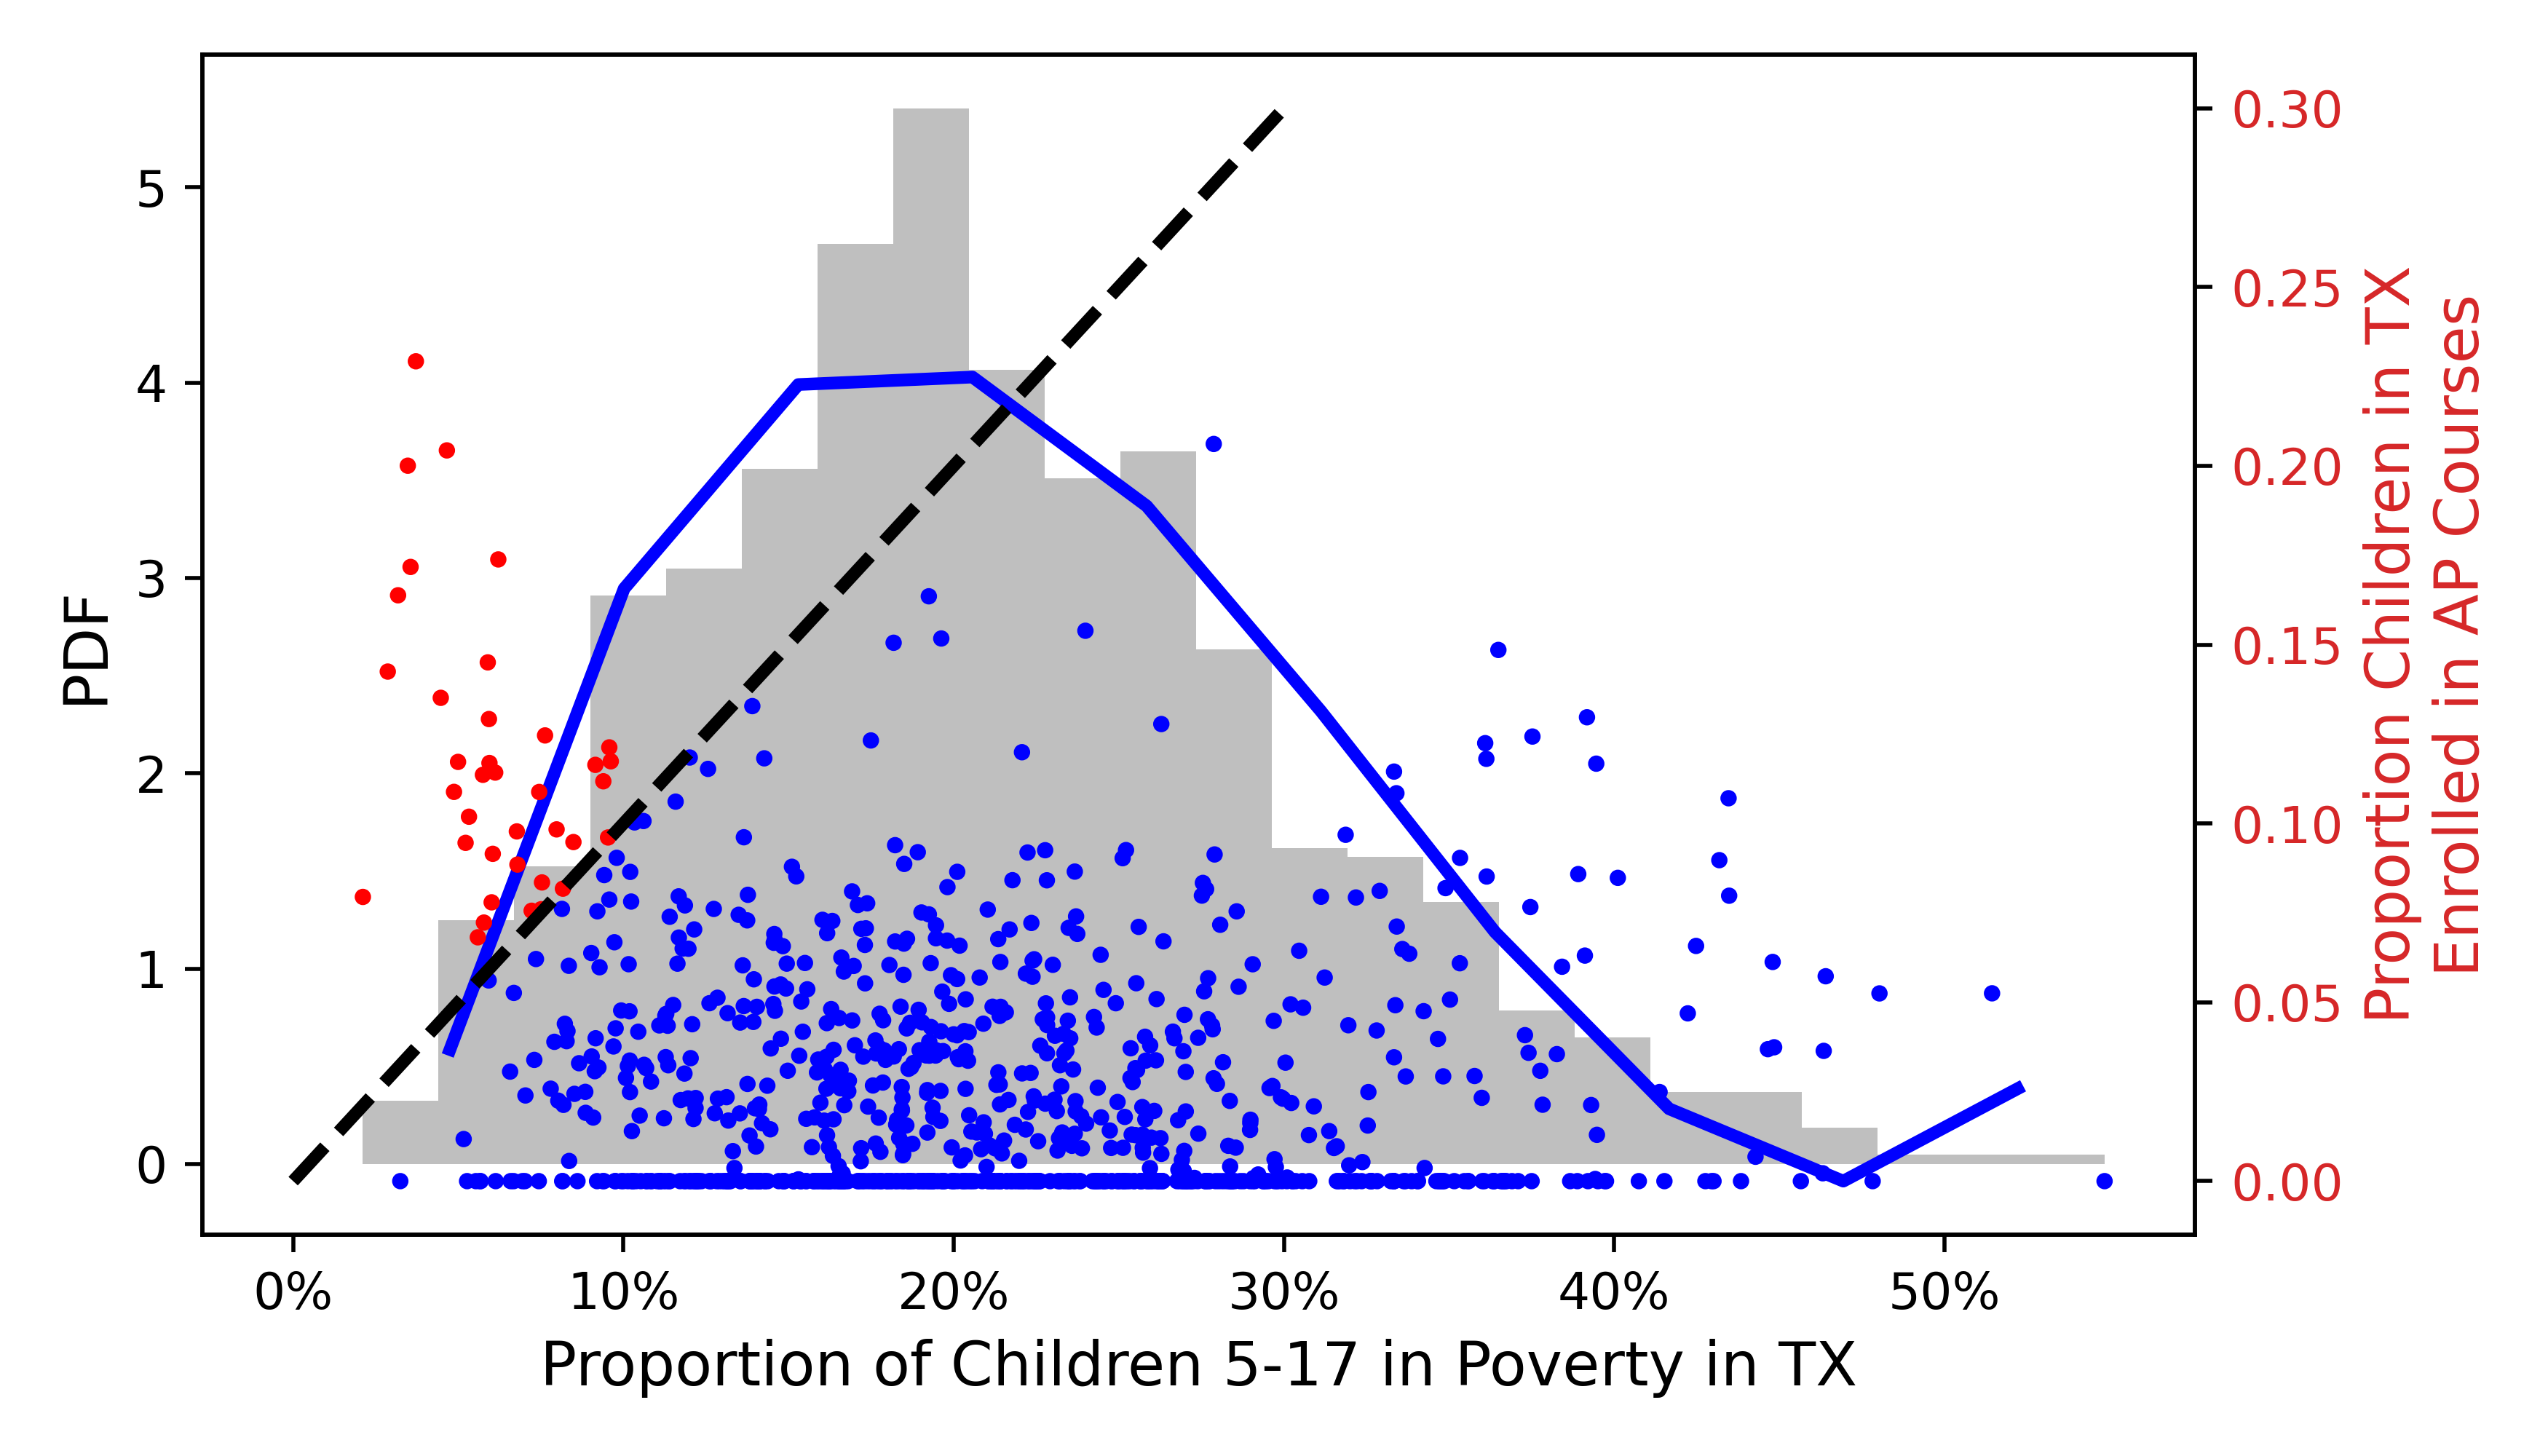
\includegraphics[]{Poverty_vs_APEnrollment_TX.png}
    \caption{Poverty vs. All AP Courses Enrollment in Texas}
    \label{fig:AP}
\end{figure}

\textbf{Correlation Insight:}\\

The scatter plot showed that most regions fall below the dashed reference line, indicating that AP courses enrollment generally lags behind poverty rates. It revealed a general trend where the proportion of children enrolled in AP courses is lower in regions with higher poverty rates. This was evidenced by the clustering of blue dots (indicating lower AP enrollment) below the black dashed reference line, particularly as poverty rates increase. This signified that in most school districts, higher poverty correlates with lower AP participation. This suggested a negative correlation between poverty and AP enrollment. As the proportion of children in poverty increases, the likelihood of lower AP courses enrollment also increased.\\

The overall negative correlation between poverty and AP courses enrollment was apparent, suggesting that higher poverty rates were associated with lower academic participation in advanced math courses. This trend underscored the challenges faced by economically disadvantaged students in accessing higher-level educational opportunities.\\

On the other hand, school districts with fewer children living in poverty (represented by the red dots) might have more resources, better funding, and more supportive environments for education, which could lead to higher enrollment in AP courses. Higher AP enrollment was often associated with better academic performance and greater access to advanced educational opportunities. This suggested that school districts with lower poverty rates tended to provide more opportunities for students to engage in advanced coursework, highlighting the positive correlation between reduced poverty and educational outcomes.\\

\textbf{Outliers:} \\

A few data points stood out as outliers. These were school districts with very high poverty rates (above 40\%) but with varying AP courses enrollment rates. These outliers highlighted extreme cases that might have been influenced by specific local factors, such as targeted educational interventions or other socioeconomic variables. The presence of these dots also suggested that certain school districts were effectively promoting AP enrollment despite socioeconomic challenges.\\

School districts with higher-than-average AP enrollment despite moderate poverty levels were indicated by the red dots above the dashed line. These school districts could provide valuable insights into effective strategies for supporting academic achievement in higher poverty contexts.\\

\textbf{Summary:}\\

The figure illustrated a significant inverse relationship between the proportion of children living in poverty and their enrollment in AP courses in Texas. While the general trend showed that higher poverty rates were associated with lower AP participation, there were exceptions where certain school districts defied this trend. These findings highlighted the need for targeted educational policies and interventions to support students in impoverished areas, aiming to bridge the gap in academic opportunities and promote equitable access to advanced coursework.\\

\subsection{AP Math Courses Enrollment vs. Poverty}

\begin{figure}[h]
    \centering
    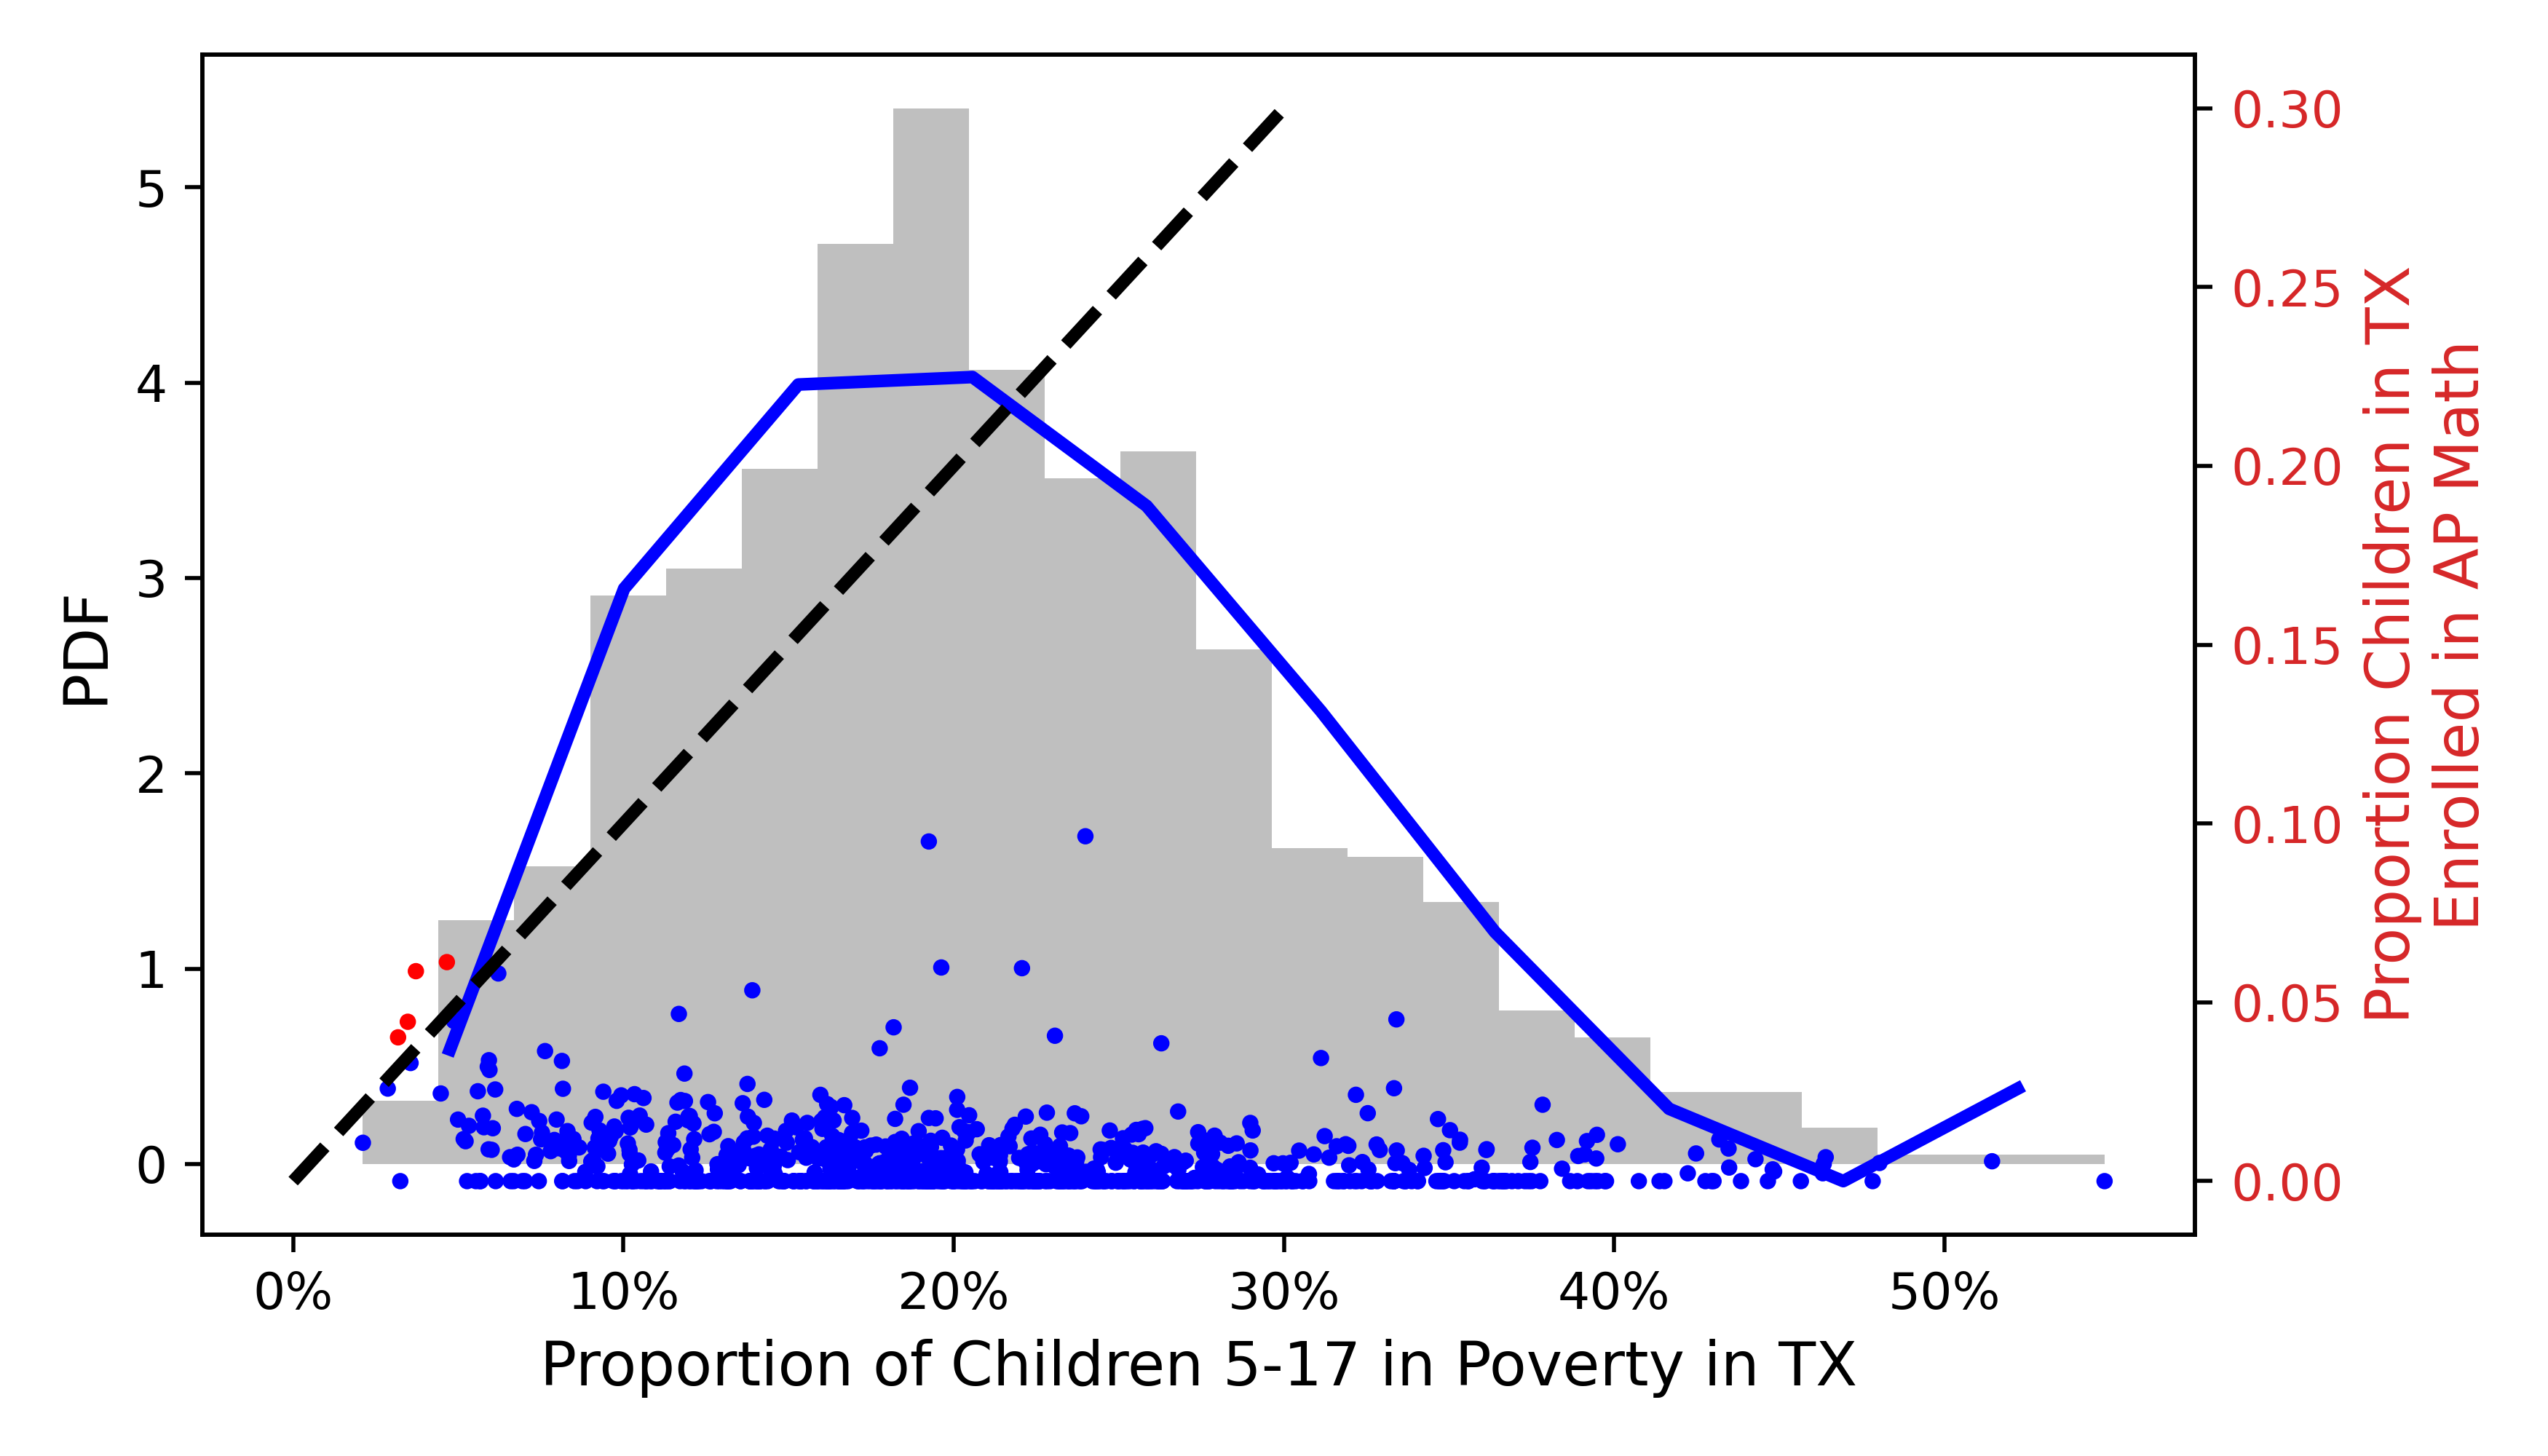
\includegraphics[]{Poverty_vs_APMath_TX.png}
    \caption{Poverty vs. AP Math Enrollment in Texas}
    \label{fig:APMath}
\end{figure}

\textbf{Correlation Insight:}\\

School districts with lower poverty rates (0\% to 10\%) exhibited a higher variance in AP Math enrollment (the red dots above the dashed reference line). As the poverty rate increased beyond 10\%, AP Math enrollment tended to decrease. Very few school districts with poverty rates above 20\% had more than 5\% of children enrolled in AP Math. The majority of blue dots lay below the black dashed line, indicating that in most school districts, the proportion of children living in poverty exceeded the proportion of children enrolled in AP Math courses.\\

This trend suggested a negative correlation between poverty rates and AP Math enrollment rates. The scatter plot demonstrated that as the proportion of children in poverty increased, the proportion of children enrolled in AP Math courses tended to decrease. Districts with higher poverty rates generally exhibited lower AP Math enrollment rates, signifying that economic disadvantage might be a significant barrier to participation in advanced academic programs.\\

\textbf{Outliers:}\\

There were a few red dots on the plot, representing school districts where the proportion of children enrolled in AP Math was higher than the proportion of children in poverty. There were few school districts with poverty rates between 20\% and 25\% that had a higher proportion of enrollment in AP Math than the school districts above the dashed line. These outliers suggested that certain school districts had effective programs or interventions that promoted AP Math enrollment despite high poverty rates. The outliers indicated that overcoming the negative impact of poverty on AP Math enrollment was possible with the right support and resources.\\

\textbf{Interesting findings:}\\

The two blue points that had higher AP Math enrollment in figure \ref{fig:APMath} are:\\

\begin{table}[h!]
\centering
\begin{tabular}{|c|c|c|c|}
\hline
\textbf{LEAID} & \textbf{School District Name} & \textbf{Poverty Proportion} & \textbf{AP Math Enrollment Proportion} \\
\hline
4814820 & Commerce ISD & 0.239886 & 0.096433 \\
\hline
4813650 & Chapel Hill ISD & 0.192478 & 0.094970 \\
\hline
\end{tabular}
\caption{Outlier Blue Points Data for TX}
\label{tab:blue_points}
\end{table}

The four school districts that were represented by the red points in figure \ref{fig:APMath} are:\\

\begin{table}[h!]
\centering
\begin{tabular}{|c|c|c|c|}
\hline
\textbf{LEAID} & \textbf{School District Name} & \textbf{Poverty Proportion} & \textbf{AP Math Enrollment Proportion} \\
\hline
4813020 & Carroll ISD & 0.031767 & 0.040206 \\
\hline
4815210 & Coppell ISD & 0.046545 & 0.061242 \\
\hline
4817760 & Eanes ISD & 0.037164 & 0.058707 \\
\hline
4828380 & Lovejoy ISD & 0.034719 & 0.044559\\
\hline
\end{tabular}
\caption{Red Points Data for TX}
\label{tab:red_points}
\end{table}

\textbf{Summary:}\\

The analysis of the data depicted in the figure highlights a concerning trend where higher poverty rates are associated with lower AP Math enrollment rates across Texas school districts. This finding underscored the impact of economic disadvantage on educational opportunities and outcomes. The negative correlation observed suggested that efforts to increase AP Math enrollment in high-poverty areas may require targeted interventions and support to overcome the barriers posed by economic hardship.\\

The analysis of the figure revealed a clear negative correlation between the proportion of children living in poverty and those enrolled in AP Math courses across Texas. While most school districts with higher poverty rates show lower AP Math enrollment, a few exceptions highlight the potential for successful educational interventions. These findings underscored the need for targeted support to boost advanced academic opportunities for students in high-poverty areas. Future research should explore the specific factors contributing to the success of outlier regions to inform policy and program development aimed at reducing educational disparities.\\
\pagebreak

\subsection{AP Science Courses Enrollment vs. Poverty}

\begin{figure}[h]
    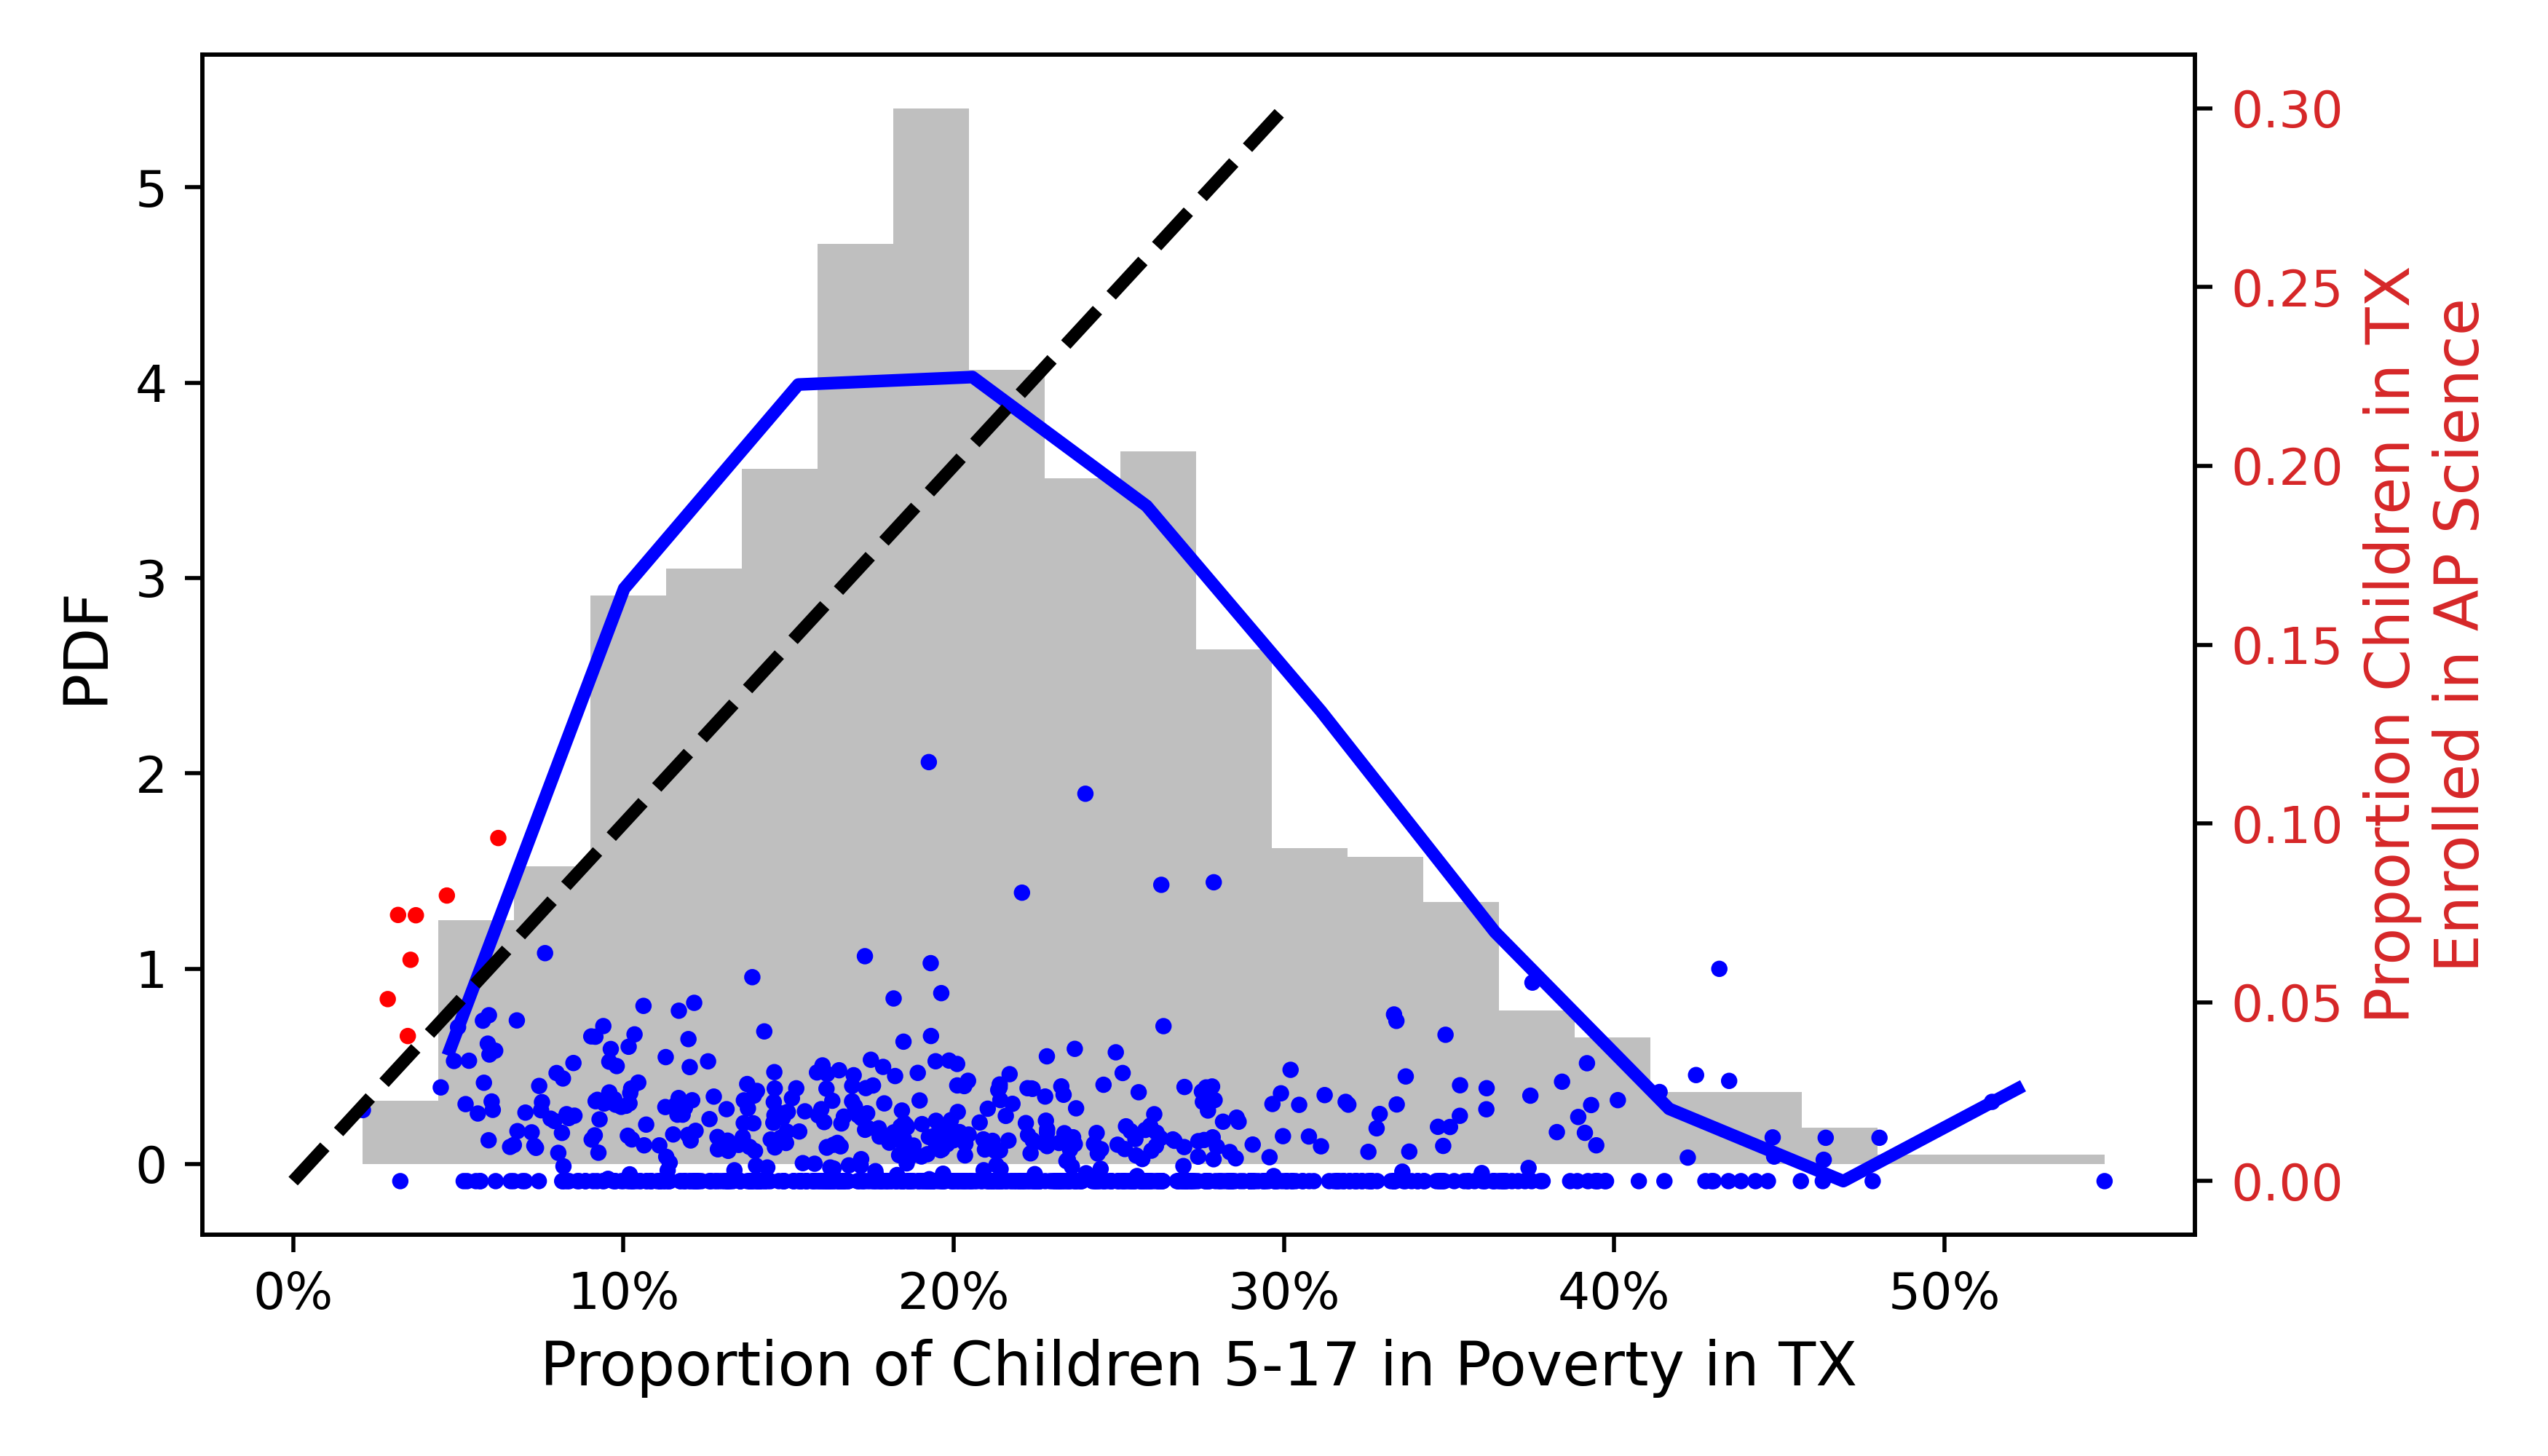
\includegraphics[]{Poverty_vs_APScience_TX.png}
    \caption{Poverty vs. AP Science Enrollment in Texas}
    \label{fig:APScience}
\end{figure}

\textbf{Correlation Insight:}\\

Similar to the trends seen in AP Math and overall AP enrollment figures, most blue dots lay below the black dashed line, indicating that in most districts, the proportion of children living in poverty exceeded the proportion enrolled in AP Science courses. This suggested a negative correlation between poverty rates and AP Science enrollment rates.\\

The scatter plot showed that as the proportion of children in poverty increased, the proportion of children enrolled in AP Science courses tended to decrease. This trend highlighted the barrier that economic disadvantage posed to participation in AP Science courses.\\
\pagebreak

\textbf{Outliers:}\\

There were a few blue dots indicating districts where AP Science enrollment met or exceeded the proportion of children in poverty. These outliers might point to districts with effective programs or policies that supported higher AP Science enrollment despite higher poverty levels.\\

\textbf{Summary:}\\

The figure revealed a significant negative correlation between the proportion of children living in poverty and the proportion enrolled in AP Science courses. As poverty rates increased, the likelihood of children enrolling in AP Science courses decreased. This pattern underscored the impact of economic disadvantage on access to advanced academic opportunities in science. Efforts to improve AP Science enrollment in high-poverty districts may require targeted support and interventions to mitigate the effects of economic hardship on educational outcomes.\\

\subsection{Compare and Contrast Across All Three Figures}

Across all three figures, there was a clear negative correlation between the proportion of children in poverty and the proportion enrolled in AP courses (All AP courses in general, AP Math and AP Science). Higher poverty rates were associated with lower enrollment rates in these advanced courses.\\

AP Math enrollment appeared to be the most negatively impacted by poverty, with the steepest decline and fewest districts overcoming this barrier. AP Science enrollment, while also negatively correlated with poverty, showed a slightly less severe decline compared to AP Math. General AP enrollment exhibited the most resilience against poverty, with more districts managing to support higher enrollment rates despite economic challenges.\\

The strong negative correlation between poverty and AP Math enrollment highlighted the need for targeted interventions to boost enrollment in advanced math courses, particularly in high-poverty districts. Strategies that have been successful in increasing general AP enrollment might be adapted and applied to improve AP Math and AP Science enrollment. Understanding the factors contributing to higher general AP enrollment in certain districts could inform policies aimed at reducing the disparity in AP Math and AP Science enrollments.\\

\textbf{Specific Observations and Comparisons}\\

The figure \ref{fig:AP} for overall AP enrollment showed more red dots, indicating more districts where overall AP enrollment met or exceeded the proportion of children in poverty. Blue dots were more spread out, indicating some districts had relatively higher overall AP enrollment rates compared to AP Math and AP Science. This suggested that while economic disadvantage impacted AP enrollment in general, districts were more successful in supporting overall AP enrollment compared to specific subjects like Math or Science.

The figure \ref{fig:APMath} for AP Math enrollment showed fewer red dots, indicating fewer districts where AP Math enrollment met or exceeded the proportion of children in poverty. Blue dots were more concentrated at the lower end of the AP Math enrollment scale, suggesting that AP Math enrollment was generally low across most districts. The slope of the decline in enrollment with increasing poverty was steep, showing a stronger negative correlation compared to other AP courses.\\

The figure \ref{fig:APScience} for AP Science enrollment showed a distribution that was somewhat intermediate between AP Math and general AP enrollment. There were more red dots compared to AP Math but fewer compared to general AP enrollment, suggesting that AP Science enrollment was less affected by poverty than AP Math but more so than overall AP enrollment. Blue dots in the AP Science figure were also spread out, similar to general AP enrollment, indicating some variability in how districts managed AP Science enrollment relative to poverty levels.\\

The presence of more red dots in figures \ref{fig:AP} (general AP) and \ref{fig:APScience} (AP Science) suggested that some districts had effective programs or policies that mitigated the association between poverty and AP enrollment. Investigating these outlier districts could provide valuable insights into successful strategies for promoting advanced coursework participation despite economic disadvantages.\\

Overall, the comparative analysis of these three figures underscored the significant association between economic disadvantage and AP course enrollment in Texas. While general AP enrollment showed some resilience, AP Math enrollment was particularly affected by poverty. Targeted interventions and policy adaptations are crucial to addressing these disparities and ensuring equitable access to advanced academic opportunities for all students.


%%%%%%%%%%%%%%%%%%%%%%%%%%%%%%%%%%%%%%%%%%%%%%%%%%%%%%%%%%%%%%
\section{Discussion}\label{sec:Discussion}

\subsection{Summary of Key Findings}

In section \ref{sec:academic}, the result examined the association between taking AP courses and various academic outcomes, including college GPA, enrollment in advanced math courses during college, and college graduation rates. The Fisher test revealed a highly significant association between taking AP courses and achieving a GPA of B or higher (p < 0.001). The odds ratio of 4.24 suggests that students who took AP courses are substantially more likely to achieve a GPA of B or higher compared to those who did not. Conversely, the relationship between taking AP courses and enrolling in advanced math courses during college showed a trend towards significance (p = 0.056), with an odds ratio of 1.08 indicating a slight increase in the likelihood of taking advanced math courses for students who took AP courses, although this result was not statistically significant. Furthermore, the Fisher test for the effect of AP courses on college graduation yielded a p-value of 0.267, indicating no significant association, with an odds ratio of 1.06 suggesting a slight but non-significant increase in the odds of graduating for students who took AP courses.\\

In section \ref{sec:socioeconomic}, the comparative analysis of the relationship between the proportion of children aged 5-17 living in poverty and enrollment in AP courses in Texas revealed significant insights into how economic disadvantage is associated with advanced academic opportunities. This study examined three specific areas of AP enrollment: overall AP courses, AP Math, and AP Science. A consistent negative correlation was observed across all figures, indicating that higher poverty rates were associated with lower AP enrollment rates. This trend highlighted the substantial barrier that economic disadvantage posed to accessing advanced coursework. The analysis of AP Math enrollment showed the steepest decline with increasing poverty, with fewer districts achieving enrollment rates that met or exceeded the proportion of children in poverty. This suggested that economic barriers had a particularly strong impact on AP Math participation. The concentration of blue dots at the lower end of the enrollment scale indicated that most districts struggled to enroll students in AP Math courses as poverty rates rose.\\

While overall AP enrollment was also negatively correlated with poverty, the effect was less severe compared to AP Math. More districts managed to support higher overall AP enrollment rates despite higher poverty levels, as indicated by the larger number of red dots. The spread of blue dots across the enrollment scale suggested variability in how districts managed overall AP enrollment relative to poverty, with some districts showing resilience against economic challenges. AP Science enrollment demonstrated a pattern that was intermediate between AP Math and overall AP enrollment. The negative correlation with poverty was evident but less pronounced than in AP Math. The presence of more red dots compared to AP Math indicated that some districts achieved higher AP Science enrollment rates despite high poverty levels, although not to the extent seen in general AP enrollment. This variability suggested that while economic disadvantage was related to AP Science enrollment, it did so to a lesser degree than AP Math, potentially due to different district-level strategies and supports.\\

Overall, these findings highlighted the critical need for equitable access to advanced academic opportunities in Texas. Economic disadvantage significantly correlated with lower AP course enrollment, particularly in math and science. By implementing targeted interventions, adapting successful strategies from general AP enrollment, and learning from high-performing districts, educational stakeholders can work towards ensuring that all students, regardless of economic background, have the opportunity to engage in and benefit from advanced coursework. This effort is vital for fostering academic excellence and preparing students for future success in higher education and beyond.\\

\subsection{Implications of Findings}

The significant positive association between AP courses and college GPA suggests that encouraging students to enroll in AP courses can enhance their academic performance in college. Choosing a GPA of B or higher as the benchmark is particularly significant because maintaining this level of academic performance can have long-term impacts on students' academic and professional trajectories. Specifically, achieving a GPA of B or higher is often a prerequisite for admission to graduate school \cite{keith-spiegel_wiederman_2000}, indicating that participation in AP courses may help students meet the rigorous academic standards required for further education beyond college. This highlights the potential long-term benefits of AP course participation, not only in terms of immediate academic performance but also in facilitating opportunities for advanced education and career advancement. Therefore, schools might consider providing more support for students to succeed in AP courses. Policymakers should also consider increasing access to AP courses, particularly for underrepresented and disadvantaged students, to help bridge the achievement gap and promote college readiness.\\

The pronounced negative correlation between poverty and AP Math enrollment highlights the need for targeted interventions to enhance participation in advanced math courses. Policies focused on providing additional resources, support programs, and tailored academic assistance are essential to address the barriers associated with economic disadvantage. By implementing such targeted support, schools can help bridge the gap and ensure that students from high-poverty backgrounds have equitable access to AP Math courses.\\

Strategies that have proven effective in boosting general AP enrollment could be adapted to support AP Math and AP Science. Understanding the factors contributing to higher overall AP enrollment in certain districts can inform policies aimed at reducing disparities in specific AP subjects. Investigating districts that have successfully achieved higher AP enrollment rates despite high poverty levels can provide valuable insights. By identifying and replicating successful programs, practices, and policies from these outlier districts, schools can create a more supportive environment for students to pursue advanced coursework in math and science, regardless of their economic background. This approach can help policymakers and educators develop more effective strategies to promote AP course enrollment across diverse socioeconomic contexts.\\

\subsection{Comparison with Previous Studies}

The findings in \ref{sub:graduation} of this study indicate no significant association between taking AP courses and college graduation rates, as evidenced by the non-significant p-value (0.267) and an odds ratio close to 1. These results suggest that the likelihood of graduating from college did not appear to be significantly associated with AP course participation during high school. These findings differ from those of several other studies reviewed in the literature. For instance, Long et al. and Ackerman et al. found a significant positive effect of AP course participation on college graduation rates \cite{ackerman2013high, long2012effects}. Long et al. reported that taking AP courses increased the likelihood of earning a bachelor’s degree within four years of high school exit by 5.0 to 8.8 percentage points \cite{long2012effects}. Similarly, Ackerman et al. found that AP course participation, coupled with earning a qualifying score of 3 or higher on AP exams, was associated with a significant increase in the likelihood of college graduation \cite{ackerman2013high}.\\

The discrepancies between this study and these previous studies could be attributed to several factors. Differences in sample size, demographic composition, institutional characteristics, and methodological approaches may all play a role. Additionally, the specific focus of AP courses (e.g., STEM vs. humanities) and the level of support provided to AP students could influence the outcomes. Further research is needed to identify the specific factors and contexts that enhance the effectiveness of AP courses in promoting college graduation.\\

In contrast, this study found a strong association between taking AP courses and achieving a GPA of B or higher, as evidenced by the highly significant p-value (p < 0.001) and an odds ratio of approximately 4.24 in \ref{sub:gpa}. These results suggest that students who took AP courses are significantly more likely to attain a GPA of B or higher compared to those who did not take AP courses.

These findings align with those of several other studies reviewed in the literature. For instance, Ackerman et al. found that participation in the AP program was associated with higher grades in post-secondary study, with a notable distinction based on the scores students achieved on AP exams. Ackerman et al. observed that students who completed larger numbers of AP exams with scores of 3 or higher tended to achieve higher first-year GPAs. Furthermore, completion of a greater number of AP exams with scores of 4 or 5 was associated with even higher first-year GPAs. For instance, students who completed at least 3 exams with scores of 3 or higher obtained a mean first-year GPA of 3.12, while those who completed at least 3 exams with scores of 4 or 5 achieved a mean GPA of 3.25. This nuanced relationship between AP exam performance and GPA underscores the importance of considering the quality and quantity of AP coursework in assessing its impact on academic outcomes.\\

While both studies underscore the positive association between AP course participation and academic success, this study provides specific insights into the likelihood of achieving a GPA of B or higher among students who took AP courses. By focusing on this specific academic benchmark, this study contributes to a nuanced understanding of the impact of AP course participation on academic outcomes. Despite the strong association found in this study, further research is needed to identify the specific factors and contexts that enhance the effectiveness of AP courses in promoting academic success, particularly in achieving higher GPAs.\\

\subsection{Limitations}

While this study provides valuable insights into the disparities in AP course enrollment across Texas school districts, several limitations should be considered when interpreting the results. The study relies on available data for the proportion of children in poverty and AP course enrollment. The accuracy and completeness of this data can vary between districts, potentially affecting the reliability of the findings. Moreover, the data does not account for other factors that might influence AP enrollment, such as school funding, teacher quality, or access to academic resources.\\

The analysis is cross-sectional, examining data from a single point in time. This approach does not capture changes over time or the potential lagged effects of poverty on AP enrollment. Longitudinal studies would provide a more comprehensive understanding of how these relationships evolve and the long-term impact of interventions. Additionally, the findings are specific to Texas and may not be generalizable to other states or regions with different demographic, economic, and educational contexts. Comparative studies across different states or regions are necessary to determine if the observed patterns hold in other contexts.\\

The study focuses on AP Math, AP Science, and overall AP enrollment, but other AP subjects, such as humanities or social sciences, were not included in the analysis. Different subjects might exhibit different enrollment patterns and relationships with poverty, which could provide a more nuanced understanding of AP disparities. Furthermore, several potential influencing factors were not examined in this study. These include the role of school leadership, parental involvement, availability of AP preparation programs, and extracurricular opportunities. A more holistic approach that considers these factors could offer a deeper understanding of the barriers and supports affecting AP enrollment.\\

The study identifies correlations between poverty and AP enrollment but does not establish causality. While the findings suggest that higher poverty rates are associated with lower AP enrollment, further research is needed to determine the causal mechanisms behind this relationship. Experimental or quasi-experimental designs could help identify the specific factors that drive these disparities. Additionally, the study does not account for the presence or absence of external support programs, such as tutoring, mentoring, or college readiness initiatives, which might influence AP enrollment. Evaluating the effectiveness of these programs could provide insights into effective strategies for mitigating the impact of poverty on AP course participation.\\

Addressing these limitations in future research would enhance the understanding of AP course enrollment disparities and inform the development of more targeted and effective interventions to promote educational equity.\\

\subsection{Future Research Directions}

The findings of this study open several avenues for future research to further understand and address the disparities in AP course enrollment across Texas school districts. One promising direction is to conduct qualitative case studies of districts that have high AP enrollment rates despite high poverty levels. By understanding the specific programs, policies, and practices implemented in these districts, valuable insights can be gained that may be adapted and applied in other contexts.\\

Another area of interest is the implementation and evaluation of targeted interventions aimed at increasing AP Math and Science enrollment in high-poverty districts. Longitudinal studies assessing the long-term effectiveness of these interventions would provide evidence-based recommendations for policymakers. Additionally, it is essential to investigate other potential barriers to AP enrollment beyond economic disadvantage, such as teacher quality, school resources, student motivation, and parental support, to design comprehensive interventions.\\

Examining the impact of teacher professional development programs on AP course enrollment and performance is another important research avenue. Understanding how training teachers to effectively teach AP courses, particularly in high-poverty schools, influences student enrollment and success can guide future professional development initiatives. Moreover, studying the impact of early academic preparation programs on later AP enrollment could reveal how initiatives at the elementary and middle school levels prepare students for the rigor of AP courses in high school, especially in math and science.\\

Investigating the role of parental and community involvement in supporting AP course enrollment can also provide valuable insights. Understanding how family and community engagement can be leveraged to support students' academic ambitions can inform holistic intervention strategies. Additionally, researching how socioeconomic factors specifically influence student performance in AP courses, including the availability of support systems, extracurricular opportunities, and access to preparatory resources, can further inform targeted interventions.\\

Extending the research to include comparative studies across different states would help identify regional differences and commonalities in AP enrollment patterns, providing a broader perspective on how state-specific policies and contexts influence AP course participation. Exploring the potential of technology and online learning platforms to increase access to AP courses in high-poverty districts is another promising area. Research could focus on the effectiveness of online AP courses and digital resources in overcoming geographic and economic barriers.\\

Finally, analyzing the impact of state and federal education policies on AP enrollment would provide insights into how legislative and funding changes influence access to and participation in advanced coursework. By pursuing these research directions, scholars and policymakers can develop a deeper understanding of the factors influencing AP course enrollment and identify effective strategies to ensure that all students, regardless of their socioeconomic status, have the opportunity to participate in and benefit from advanced academic programs.\\

In addition to examining enrollment patterns, future research should explore the long-term effects of AP course participation on post-college outcomes, such as career success and graduate school enrollment. Studies should also examine the impact of AP courses across different demographic groups and educational contexts to better understand the conditions under which AP courses are most beneficial. Conducting qualitative research, such as interviews with students and educators, could provide deeper insights into the mechanisms through which AP courses influence academic success. Integrating these broader outcome measures and qualitative insights with the current focus on enrollment disparities will offer a comprehensive understanding of the role of AP courses in promoting educational equity and excellence.\\

%%%%%%%%%%%%%%%%%%%%%%%%%%%%%%%%%%%%%%%%%%%%%%%%%%%%%%%%%%%%%%
\section{Conclusion}\label{sec13}

This thesis has explored the impact of Advanced Placement (AP) course participation on various academic outcomes and the relationship between socioeconomic status and AP course enrollment across Texas. Through an analysis of data from the Civil Rights Data Collection (CRDC), the U.S. Census Bureau’s Small Area Income and Poverty Estimates (SAIPE) program, and the University of Texas at San Antonio, the findings from this study offer several important insights into the opportunity gap and educational equity.\\

In conclusion, this thesis underscores the critical importance of addressing the opportunity gap to promote educational equity and excellence. By implementing targeted interventions and fostering a supportive and inclusive educational environment, we can ensure that all students, regardless of their socioeconomic background, have the opportunity to achieve their full potential and succeed in their academic and professional pursuits.\\

Every student is taught that ``education equals opportunity", and we hope that in the near future, this belief will fully reflect reality. One day, no one should be able to predict a student's success based on their race, zip code, school name, school district, or their parents' socioeconomic status.

\backmatter

\bmhead{Supplementary information}

Mention to a github repository

\bmhead{Acknowledgements}

There is no funding associated with this research. 

\section*{Declarations}

\begin{itemize}
\item Funding: None.
\item Conflict of interest/Competing interests: None.
\item Ethics approval and consent to participate: Not applicable.
\item Consent for publication. Not applicable. 
\item Data availability: Public data sources as detailed in the methods section.  
\item Materials availability: Not applicable.
\item Code availability: Git hub repository...
\item Author contribution: KH wrote the manuscript as her M.Sc. Thesis under the direction of JBG. TV and PP were part of the thesis committee, reviewed the mansucript and provided feedback during preparation of the thesis and submission of the article. 
\end{itemize}

\noindent
If any of the sections are not relevant to your manuscript, please include the heading and write `Not applicable' for that section. 

%%===================================================%%
%% For presentation purpose, we have included        %%
%% \bigskip command. Please ignore this.             %%
%%===================================================%%
\bigskip
\begin{flushleft}%
Editorial Policies for:

\bigskip\noindent
Springer journals and proceedings: \url{https://www.springer.com/gp/editorial-policies}

\bigskip\noindent
Nature Portfolio journals: \url{https://www.nature.com/nature-research/editorial-policies}

\bigskip\noindent
\textit{Scientific Reports}: \url{https://www.nature.com/srep/journal-policies/editorial-policies}

\bigskip\noindent
BMC journals: \url{https://www.biomedcentral.com/getpublished/editorial-policies}
\end{flushleft}

\begin{appendices}

\section{Section title of first appendix}\label{secA1}

An appendix contains supplementary information that is not an essential part of the text itself but which may be helpful in providing a more comprehensive understanding of the research problem or it is information that is too cumbersome to be included in the body of the paper.

%%=============================================%%
%% For submissions to Nature Portfolio Journals %%
%% please use the heading ``Extended Data''.   %%
%%=============================================%%

%%=============================================================%%
%% Sample for another appendix section			       %%
%%=============================================================%%

%% \section{Example of another appendix section}\label{secA2}%
%% Appendices may be used for helpful, supporting or essential material that would otherwise 
%% clutter, break up or be distracting to the text. Appendices can consist of sections, figures, 
%% tables and equations etc.

\end{appendices}

%%===========================================================================================%%
%% If you are submitting to one of the Nature Portfolio journals, using the eJP submission   %%
%% system, please include the references within the manuscript file itself. You may do this  %%
%% by copying the reference list from your .bbl file, paste it into the main manuscript .tex %%
%% file, and delete the associated \verb+\bibliography+ commands.                            %%
%%===========================================================================================%%

\bibliography{sn-bibliography}% common bib file
%% if required, the content of .bbl file can be included here once bbl is generated
%%\input sn-article.bbl


\end{document}
